\documentclass[letterpaper, 10pt, oneside, twocolumn, final]{article}
% * <leofangxh@gmail.com> 2017-12-07T09:31:12.972Z:
%
% ^.
\usepackage{caption}
\DeclareCaptionFont{blue}{\color{blue}}
\captionsetup{labelfont={blue,footnotesize},textfont={blue,footnotesize}}
\usepackage{amsmath} %Allows use of multline and align options
\usepackage[amssymb]{SIunits}
\usepackage{amssymb}
%\pagestyle{empty}%No page numbers
\usepackage[twocolumn,top=0.5in,bottom=0.5in,left=0.5in,textwidth=7.5in,columnsep=0.5in]{geometry}
\usepackage{parskip}
 \usepackage{nopageno}
\usepackage{graphicx}
\usepackage{color}
\usepackage{subfigure}
%\usepackage{subcaption}
\usepackage{appendix}
\usepackage{float}
\usepackage{pbox}
\usepackage{tabu}
\usepackage{tabularx}
\usepackage{longtable}
\usepackage{supertabular,booktabs}
% * <leofangxh@gmail.com> 2017-10-23T11:33:36.071Z:
%
% ^.
\usepackage{array}
\usepackage{multirow}
\usepackage{wrapfig}
%\usepackage[none]{hyphenat}
%\usepackage{subfig}   % use subfigures
\usepackage{authblk}  %multiple authors
\usepackage{fancyhdr} % fancy headers
\usepackage[compact]{titlesec} % section headings
\usepackage{natbib}
\usepackage[table]{xcolor} % table, coloured rows
%\usepackage{setspace}
\usepackage[labelfont=bf, labelsep=period]{caption}
%nomenclature stuff

\usepackage{nomencl}%nomen
\setlength{\nomitemsep}{-\parsep}
\setlength{\columnsep}{3em}
\makenomenclature

%\usepackage[version=3]{mhchem} % chemical reaction environment
%\usepackage[%
%  obeyall,
%  repeatunits=false,
%  trapambigrange=false]{siunitx}  % typesetting units
% %% Plotting, PGF and tikz graphics
\usepackage{tikz,tikz-3dplot}
%\usetikzlibrary{shapes.geometric,backgrounds,positioning-plus,node-families,calc}
\usetikzlibrary{shapes, quotes}
\usetikzlibrary{patterns}
\usetikzlibrary{automata,positioning}
% %\usetikzlibrary{external}
 %\tikzexternalize[prefix=tikz/]
 \usetikzlibrary{matrix}
\usepackage{pgfplots,pgfplotstable}
\usepgfplotslibrary{groupplots}
\usepgfplotslibrary{fillbetween}
 \usepackage{scalefnt}
 \pgfplotsset{compat=newest}
 \usepackage{filecontents}
 \usepackage{caption}
% fonts
\usepackage[T1]{fontenc}
\usepackage{mathptmx}
\usepackage{titlesec}
\usepackage{mwe,tikz}\usepackage[percent]{overpic}
\usepgfplotslibrary{patchplots}
\usepgfplotslibrary{units}
\usepgfplotslibrary{fillbetween}
\usepgfplotslibrary{groupplots}
\pgfplotsset{
	/pgfplots/colormap={jet}{rgb255(0cm)=(0,0,128) rgb255(1cm)=(0,0,255)
		rgb255(3cm)=(0,255,255) rgb255(5cm)=(255,255,0) rgb255(7cm)=(255,0,0)
		rgb255(8cm)=(128,0,0)},
		% erdc rainbow dark
	colormap={erdc_dk}{
		rgb=(0.000000, 0.000000, 0.423499) 
		rgb=(0.000000, 0.119346, 0.529237) 
		rgb=(0.000000, 0.238691, 0.634976) 
		rgb=(0.000000, 0.346852, 0.687880) 
		rgb=(0.000000, 0.450220, 0.718141) 
		rgb=(0.000000, 0.553554, 0.664839) 
		rgb=(0.000000, 0.651082, 0.519303) 
		rgb=(0.115841, 0.724790, 0.352857) 
		rgb=(0.326771, 0.781195, 0.140187)
		rgb=(0.522765, 0.798524, 0.028462) 
		rgb=(0.703162, 0.788685, 0.008858) 
		rgb=(0.845118, 0.751133, 0.000000) 
		rgb=(0.955734, 0.690825, 0.000000) 
		rgb=(0.995402, 0.567916, 0.061852) 
		rgb=(0.987712, 0.403398, 0.164851) 
		rgb=(0.980407, 0.247105, 0.262699)
	},
	% erdc rainbow light
	colormap={erdc_lt}{
		rgb=(0.325490, 0.149020, 0.960784) 
		rgb=(0.297047, 0.375586, 0.963836) 
		rgb=(0.180302, 0.536818, 0.964627) 
		rgb=(0.130200, 0.649207, 0.929647) 
		rgb=(0.044514, 0.749654, 0.855998) 
		rgb=(0.027133, 0.830713, 0.721527) 
		rgb=(0.259504, 0.866145, 0.543555) 
		rgb=(0.428364, 0.890725, 0.329819) 
		rgb=(0.568503, 0.898508, 0.187623)
		rgb=(0.738259, 0.890317, 0.082546) 
		rgb=(0.845460, 0.861360, 0.014755) 
		rgb=(0.912191, 0.808018, 0.000000) 
		rgb=(0.962848, 0.710445, 0.000000) 
		rgb=(0.999469, 0.600258, 0.017628) 
		rgb=(0.994156, 0.445975, 0.193912) 
		rgb=(0.980407, 0.247105, 0.262699)
	},
	%spectral
	colormap={spectral}{
		rgb=(0.368627, 0.309804, 0.635294)
		rgb=(0.260361, 0.450058, 0.701730)
		rgb=(0.248058, 0.591311, 0.717186)
		rgb=(0.376009, 0.734025, 0.658132) 
		rgb=(0.537947, 0.814764, 0.645060) 
		rgb=(0.702345, 0.879585, 0.636678) 
		rgb=(0.847520, 0.938639, 0.607151) 
		rgb=(0.940408, 0.976163, 0.656055) 
		rgb=(0.999923, 0.997616, 0.745021) 
		rgb=(0.997463, 0.921338, 0.617070) 
		rgb=(0.995002, 0.824606, 0.499885) 
		rgb=(0.992541, 0.701576, 0.396540) 
		rgb=(0.973472, 0.547405, 0.318108) 
		rgb=(0.937793, 0.398539, 0.270127) 
		rgb=(0.861515, 0.282891, 0.299654) 
		rgb=(0.746482, 0.144637, 0.288812) 
		rgb=(0.619608, 0.003922, 0.258824)	
	},
every axis/.append style={
	label style={font=\small},
	tick label style={font=\footnotesize},
	xtick style={color=black},
	ytick style={color=black},
	minor tick num=5,
	legend style={font=\footnotesize},
},
}
\pgfplotsset{every axis/.append style={
		label style={font=\small},
		tick label style={font=\footnotesize},
		xtick style={color=black},
		ytick style={color=black},
		minor tick num=5,
		legend style={font=\footnotesize},
}}
%% Some extra plot colors 
\definecolor{Set1-6-1}{RGB}{228,26,28}
\definecolor{Set1-6-2}{RGB}{55,126,184}
\definecolor{Set1-6-3}{RGB}{77,175,74}
\definecolor{Set1-6-4}{RGB}{152,78,163}
\definecolor{Set1-6-5}{RGB}{255,127,0}
\definecolor{Set1-6-6}{RGB}{255,255,51}
\definecolor{RdGy-4-1}{RGB}{202,0,32}
\definecolor{RdGy-4-4}{RGB}{64,64,64}
\definecolor{RdBu-4-4}{RGB}{5,113,176}
\definecolor{RdPu-3-3}{RGB}{197,27,138}
\definecolor{PRGn-4-1}{RGB}{123,50,148}
\definecolor{PRGn-4-4}{RGB}{0,136,55}
\definecolor{BrBG-4-1}{RGB}{166,97,26}
\definecolor{Oranges-3-3}{RGB}{230,85,13}
\definecolor{YlGn-4-4}{RGB}{35,132,67}

\setcounter{secnumdepth}{4}


% pdf/dvips specific includes
\usepackage{ifpdf}
\ifpdf
\usepackage{epstopdf}
\usepackage[pdftex]{hyperref}
\else
\usepackage[dvips]{hyperref}
\fi
\newcommand\Tstrut{\rule{0pt}{2.6ex}}         % = `top' strut
\newcommand\Bstrut{\rule[-0.9ex]{0pt}{0pt}}   % = `bottom' strut

% setup hypperref
\hypersetup{ 
	colorlinks=true, 
	linkcolor=black, 
	citecolor=black,
	filecolor=black, 
	urlcolor=black, 
	bookmarksnumbered=true,
	breaklinks=true }


%% replace itemize by squishlist (saves space)
\newcommand{\squishlist}{
	\begin{list}{$\bullet$}
		{ \setlength{\itemsep}{0pt}
			\setlength{\parsep}{3pt}
			\setlength{\topsep}{3pt}
			\setlength{\partopsep}{0pt}
			\setlength{\leftmargin}{1.5em}
			\setlength{\labelwidth}{1em}
			\setlength{\labelsep}{0.5em} } }
	
	\newcommand{\squishlisttwo}{
		\begin{list}{$\bullet$}
			{ \setlength{\itemsep}{0pt}
				\setlength{\parsep}{0pt}
				\setlength{\topsep}{0pt}
				\setlength{\partopsep}{0pt}
				\setlength{\leftmargin}{2em}
				\setlength{\labelwidth}{1.5em}
				\setlength{\labelsep}{0.5em} } }
		
		\newcommand{\squishend}{
	\end{list}  }
	
	% Alter some LaTeX defaults for better treatment of figures:
	\renewcommand{\topfraction}{0.9} % max fraction of floats at top
	\renewcommand{\bottomfraction}{0.9} % max fraction of floats at bottom
	\renewcommand{\textfraction}{0.1} % allow minimal text w. figs
	\renewcommand{\floatpagefraction}{0.9} % require fuller float pages
	\renewcommand{\dbltopfraction}{0.9} % fit big float above 2-col. text
	\renewcommand{\dblfloatpagefraction}{0.9} % require fuller float pages
	\setcounter{topnumber}{2}
	\setcounter{bottomnumber}{2}
	\setcounter{totalnumber}{4}
	\setcounter{dbltopnumber}{2}
	%---------------------------------------------------------------------
	% style
	
	% bibliography spacing
	\setlength{\bibsep}{0pt}
	
	%% newcommands for maths symbols
	\newcommand{\pfrac}[2]{\frac{\partial{#1}}{\partial{#2}}}
	\newcommand{\vp}{\ensuremath \varphi }
	\newcommand{\p}{\ensuremath \phi}
	\newcommand{\z}{\ensuremath Z}
	\newcommand{\yc}{\ensuremath $Y_c$}
	\newcommand{\2}{\ensuremath $_2$}
	\newcommand{\ch}{\ensuremath CH$_4$}
	\newcommand{\w}{\ensuremath \omega}
	\newcommand{\et}{{\em et al.}}
	
	% section headings
	\titleformat*{\section}{\normalsize\bfseries}
	\titleformat*{\subsection}{\normalsize\bfseries}
	\titleformat*{\subsubsection}{\normalsize\bfseries}
	\titlespacing*{\section}{0pt}{3.25ex plus 1ex minus .2ex}{1.5ex plus .2ex}
	\titlespacing*{\subsection}{0pt}{3.25ex plus 1ex minus .2ex}{1.5ex plus .2ex}
	\titlespacing*{\subsubsection}{0pt}{3.25ex plus 1ex minus .2ex}{1.5ex plus .2ex}
	\makeatletter
	\def\@seccntformat#1{\@ifundefined{#1@cntformat}%
		{\csname the#1\endcsname\quad}% default
		{\csname #1@cntformat\endcsname}}% individual control
	\def\section@cntformat{\thesection.\quad}
	\makeatother
	
	% set the frame style for fbox
	\setlength\fboxsep{0pt}
	\setlength\fboxrule{0.5pt}
	\newcommand{\mybox}[1]{#1}
	
	\newcounter{mylistctr}
	
	%% Shortcut commands
	\newcommand{\rrate}{\ensuremath {\dot{\omega}}}
	%\newcommand{\etal}{{\em et al}.}
%\makeatletter
%\renewcommand*{\@biblabel}[1]{\hfill#1.}
%\makeatother
\begin{document}
\pagenumbering{gobble} 	
	\twocolumn[
	\begin{@twocolumnfalse}
		\begin{flushright}
			\small{\bf{2020-01-XXXX}}\\ \vspace{16pt}
			\Large{\bf{Sample Plot For Latex}}\\ \vspace{16pt}
			\large{\bf{X.H. Fang}}\\ 
			\normalsize{Department of Engineering Science, University of Oxford, UK}\\\vspace{16pt}
		\end{flushright}
		{\footnotesize Copyright \copyright~\the\year~SAE International }\vspace{36pt}
	\end{@twocolumnfalse}
	]
	
\raggedright


%%%%%%%%%%%%%%%%%%%%%%%%%%%%%%%%%%%%%%%%%%%%%%%%%%%%%%%%%%%%%%%%%%%%%%%%%%%%%%%%%%%%%%%%%%%%%%%%%%%%%%%%%%%%%%%%%%%%%%%%%%%%
\section*{Flamelet Plots}


\begin{figure}[h]
	\centering
	\begin{tikzpicture}[scale=1,>=latex]%
	\begin{axis}%
	[%
	ylabel=Temperature {[K]},
	xlabel=x {[cm]},
	width=10cm, height=8cm,
	xmin = -0.04, xmax = 0.04,
	ymin =363, ymax = 2400,
	xticklabel style={
		/pgf/number format/fixed,
		/pgf/number format/precision=2,
		/pgf/number format/fixed zerofill
	},
	scaled x ticks=false,
	%xtick distance={0.2}, ytick distance={0.1},
	legend style={line width=1.5pt, draw =none, legend pos=north east,fill=none, legend cell align=left}, 
	line width=1.0pt %
	]%
	%% Plot stuff
	\addplot [dotted, color={RdGy-4-4},forget plot] table{figures/flamelet_xt/xtemp_yi00000800.dat};		
	\addplot [dotted, color={RdGy-4-4},forget plot] table{figures/flamelet_xt/xtemp_yi00001500.dat};
	\addplot [dotted, color={RdGy-4-4},forget plot] table{figures/flamelet_xt/xtemp_yi00001800.dat};
	\addplot [dotted, color={RdGy-4-4},forget plot] table{figures/flamelet_xt/xtemp_yi00002000.dat};
	\addplot [dotted, color={RdGy-4-4},forget plot] table{figures/flamelet_xt/xtemp_yi00002400.dat};
	\addplot [dotted, color={RdGy-4-4},forget plot] table{figures/flamelet_xt/xtemp_yi00002800.dat};
	%\addplot [dotted, color={RdGy-4-4},forget plot] table{figures/flamelet_xt/xtemp_yi00003200.dat};
	%\addplot [dotted, color={RdGy-4-4},forget plot] table{figures/flamelet_xt/xtemp_yi00004000.dat};
	%\addplot [dotted, color={RdGy-4-4},forget plot] table{figures/flamelet_xt/xtemp_yi00005000.dat};
	%\addplot [dotted, color={RdGy-4-4},forget plot] table{figures/flamelet_xt/xtemp_yi00006200.dat};
	\addplot [dashed, color={RdGy-4-1},forget plot] table{figures/flamelet_xt/xtemp_yi00006460.dat};

	\addplot [smooth, color={YlGn-4-4},forget plot] table{figures/flamelet_xt/xtemp_yistart.dat};
	
	\draw [dashed, thick] (0,363) to (0,1900);
	\node at (0.015,1400) {Stagnation plane};
	
	\draw [->, thick] (-0.0075,500) to (-0.02,2200);
	\node at (-0.0225,500) {Time advancement};	
	
	
	\addlegendimage{color={YlGn-4-4},smooth}
	\addlegendentry{Mixing solution}
	\addlegendimage{color={RdGy-4-4},dotted}
	\addlegendentry{Transient solutions}
	\addlegendimage{color={RdGy-4-1},dashed}
	\addlegendentry{Quasi steady state solution}
	\end{axis}
	
	\end{tikzpicture}
	\caption{Temperature evolution in space, $x$ and time, $t$ for an igniting counter-flow diffusion flame with N-dodecane: $a=500$ s$^{-1}$, $T_{fu}=363$ K, $T_{ox}=800$ K, $P_{amb}=5.25$ MPa, $\mathsf{O_{2}}=15$ \%.}
	\label{fig:icdf_Txt}
\end{figure}



\begin{figure}[h]
	\centering
	\begin{tikzpicture}[scale=1, >=latex]%
	\begin{axis}%
	[%
	ylabel=Temperature {[K]},
	xlabel=Mixture fraction{,} $Z$ {[-]},
	width=10cm, height=8cm, 
	xmin = 0, xmax = 1,
	ymin =363, ymax = 2400,
	%xtick distance={0.2}, ytick distance={0.1},
	legend style={draw =none, legend pos=north east,fill=none, legend cell align=left}, 
	line width=1.0pt %
	]%
	%% Plot stuff
	\addplot [dotted, color={RdGy-4-4},forget plot] table{figures/flamelet_xt/xz_yi00000800.dat};
	\addplot [dotted, color={RdGy-4-4},forget plot] table{figures/flamelet_xt/xz_yi00001000.dat};
	\addplot [dotted, color={RdGy-4-4},forget plot] table{figures/flamelet_xt/xz_yi00001500.dat};
	\addplot [dotted, color={RdGy-4-4},forget plot] table{figures/flamelet_xt/xz_yi00001800.dat};
	\addplot [dotted, color={RdGy-4-4},forget plot] table{figures/flamelet_xt/xz_yi00002000.dat};
	\addplot [dotted, color={RdGy-4-4},forget plot] table{figures/flamelet_xt/xz_yi00002400.dat};
	\addplot [dotted, color={RdGy-4-4},forget plot] table{figures/flamelet_xt/xz_yi00002800.dat};
	%\addplot [dotted, color={RdGy-4-4},forget plot] table{figures/flamelet_xt/xz_yi00003200.dat};
	%\addplot [dotted, color={RdGy-4-4},forget plot] table{figures/flamelet_xt/xz_yi00004000.dat};
	%\addplot [dotted, color={RdGy-4-4},forget plot] table{figures/flamelet_xt/xz_yi00005000.dat};
	%\addplot [dotted, color={RdGy-4-4},forget plot] table{figures/flamelet_xt/xz_yi00006200.dat};
	\addplot [dashed, color={RdGy-4-1},forget plot] table{figures/flamelet_xt/xz_yi00006460.dat};
	
	\addplot [smooth, color={YlGn-4-4},forget plot] table{figures/flamelet_xt/xz_yistart.dat};
	
	\draw [->, thick] (0.18,600) to (0.065,2200);
	\node at (0.26,1900) {Time advancement};
	
	\draw [-, thick] (0.045,363) to (0.045,2400);
	\node at (0.075,500) {$Z_{st}$};
	
	\addlegendimage{color={YlGn-4-4},smooth}
	\addlegendentry{Mixing solution}
	\addlegendimage{color={RdGy-4-4},dotted}
	\addlegendentry{Transient solutions}
	\addlegendimage{color={RdGy-4-1},dashed}
	\addlegendentry{Quasi steady state solution}
	
	\end{axis}
	
	\end{tikzpicture}
	\caption{Temperature evolution in mixture fraction space for an igniting counter-flow diffusion flame with N-dodecane: $a=500$ s$^{-1}$, $T_{fu}=363$ K, $T_{ox}=800$ K, $P_{amb}=5.25$ MPa, $\mathsf{O_{2}}=15$ \%.}
	\label{fig:icdf_Tz}
\end{figure}

\begin{figure}[h]
	\centering
	\begin{tikzpicture}[scale=1,>=latex]%
	\begin{axis}%
	[%
	ylabel=Progress variable{,} $\mathcal{C}$ {[-]},
	xlabel=Mixture fraction{,} $Z$ {[-]},
	width=10cm, height=8cm, 
	xmin = 0, xmax = 1,
	ymin =0, ymax = 0.3,
	xtick distance={0.2}, ytick distance={0.1},
	legend style={draw =none, legend pos=north east,fill=none, legend cell align=left}, 
	line width=1.0pt %
	]%
	%% Plot stuff
	\addplot [dashed, color={RdGy-4-1},forget plot] table{figures/manifoldgen/scdf_1.dat};
	
	\addplot [dashed, color={RdGy-4-1},forget plot] table {figures/manifoldgen/scdf_5.dat};
	\addplot [dashed, color={RdGy-4-1},forget plot] table {figures/manifoldgen/scdf_52.dat};
	\addplot [dashed, color={RdGy-4-1},forget plot] table {figures/manifoldgen/scdf_500.dat};
	
	\addplot [dotted, color={RdGy-4-4},forget plot] table {figures/manifoldgen/icdf_t800.dat};
	\addplot [dotted, color={RdGy-4-4},forget plot] table {figures/manifoldgen/icdf_t1200.dat};
	\addplot [dotted, color={RdGy-4-4},forget plot] table {figures/manifoldgen/icdf_t1500.dat};
	\addplot [dotted, color={RdGy-4-4},forget plot] table {figures/manifoldgen/icdf_t1600.dat};
	\addplot [dotted, color={RdGy-4-4},forget plot] table {figures/manifoldgen/icdf_t1800.dat};
	\addplot [dotted, color={RdGy-4-4},forget plot] table {figures/manifoldgen/icdf_t2000.dat};
	\addplot [dotted, color={RdGy-4-4},forget plot] table {figures/manifoldgen/icdf_t2400.dat};
	\addplot [dotted, color={RdGy-4-4},forget plot] table {figures/manifoldgen/icdf_t2800.dat};
	
	\addplot [smooth, color={YlGn-4-4},forget plot] table{figures/manifoldgen/mixingsol.dat};
	
	\addlegendimage{color={YlGn-4-4},smooth}
	\addlegendentry{Mixing solution}
	\addlegendimage{color={RdGy-4-4},dotted}
	\addlegendentry{Igniting solutions: $a=500$ s$^{-1}$}
	\addlegendimage{color={RdGy-4-1},dashed}
	\addlegendentry{Steady solutions: $a=500$...$1$ s$^{-1}$}
	
	\draw [->, thick] (0.4,0.125) to (0.5,0.18);
	\node at (0.725,0.175) {Decreasing strain rate};
	
	\end{axis}
	
	\end{tikzpicture}
	\caption{Schematic representation of progress variable as a function of mixture fraction for a series of counter-flow diffusion flamelets.}
	\label{fig:pvz_space}
\end{figure}





\section*{2D line plot}


%%%%%%%%%%%%%%%%%%%%%%%%%%%%%%%Begin Figure%%%%%%%%%%%%%%%%%%%%%%%%%%%%%%
\begin{figure}
    \centering
   

\begin{tikzpicture}
\begin{axis}[
    %xtick={1000,20,40,60,80,100},
    %ytick={0,10,20,30,35},
    %minor tick style={draw=none}
    %yminortick=none;
    %legend pos=north west,
    %ymajorgrids=true,
    %grid style=dashed,
    scale=0.8,
    axis y line*=left,
    enlargelimits=false,
	width=8cm, height=6cm,
	scale only axis,
	xlabel={$y$ [mm]},
	ylabel={Temperature [K]},
	xmin = -5, xmax = 5,
	ymin = 750, ymax = 1500,
	xtick distance={1},
	ytick distance={200},
	legend style={legend pos=north west,legend cell align=left}
]
\addplot[
    smooth,
    thick,
    color={RdBu-4-4},
    ]
table[x index = {0}, y index = {1}] 
{figures/chi/95atemp.txt};
\addlegendentry{Temperature}
\node[text=black] at (3, 1330) {{0.95 ms (A)}};


\end{axis}

\begin{axis}[
    %xtick={1000,20,40,60,80,100},
    %ytick={0,10,20,30,35},
    %minor tick style={draw=none}
    %yminortick=none;
    %legend pos=north west,
    %ymajorgrids=true,
    %grid style=dashed,
    enlargelimits=false,
    scale=0.8,
	width=8cm, height=6cm,
	scale only axis,
	axis y line*=right,
	ylabel={\textcolor{Set1-6-3}{$\chi$ [1/s]}},
	xmin = -5, xmax = 5,
	ymin = -5, ymax = 50,
 	ytick distance={10},
%  	yticklabels={\textcolor{Set1-6-3}{-300},\textcolor{Set1-6-3}{-200},\textcolor{Set1-6-3}{-100},\textcolor{Set1-6-3}{0},\textcolor{Set1-6-3}{100},\textcolor{Set1-6-3}{200},\textcolor{Set1-6-3}{300},\textcolor{Set1-6-3}{400},\textcolor{Set1-6-3}{500},\textcolor{Set1-6-3}{600}}
	legend style={legend pos=north east,legend cell align=left}
]
\addplot[
    dashed,
    thick,
    color={Oranges-3-3},
    mark size=2.5 pt]
table[x index = {0}, y index = {1}] 
{figures/chi/95achi.txt};
\addlegendentry{\textcolor{BrBG-4-1}{$\chi$}}
\end{axis}

\end{tikzpicture}

    
\end{figure}
%%%%%%%%%%%%%%%%%%%%%%%%%%%%%%%End Figure%%%%%%%%%%%%%%%%%%%%%%%%%%%%%%








%%%%%%%%%%%%%%%%%%%%%%%%%%%%%%%Begin Figure%%%%%%%%%%%%%%%%%%%%%%%%%%%%%%
\begin{figure}
    \centering
   

\begin{tikzpicture}
\begin{axis}[
    %xtick={1000,20,40,60,80,100},
    %ytick={0,10,20,30,35},
    %minor tick style={draw=none}
    %yminortick=none;
    %legend pos=north west,
    %ymajorgrids=true,
    %grid style=dashed,
    scale=0.8,
        axis y line*=left,
    enlargelimits=false,
	width=8cm, height=6cm,
	scale only axis,
	xlabel={$y$ [mm]},
	ylabel={Temperature [K]},
	xmin = -5, xmax = 5,
	ymin = 750, ymax = 1500,
	xtick distance={1},
	ytick distance={200},
	legend style={legend pos=north west,legend cell align=left}
]
\addplot[
    smooth,
    thick,
    color={RdBu-4-4},
    ]
table[x index = {0}, y index = {1}] 
{figures/chi/97atemp.txt};
\addlegendentry{Temperature}
\node[text=black] at (3, 1330) {{0.97 ms (B)}};

\end{axis}

\begin{axis}[
    %xtick={1000,20,40,60,80,100},
    %ytick={0,10,20,30,35},
    %minor tick style={draw=none}
    %yminortick=none;
    %legend pos=north west,
    %ymajorgrids=true,
    %grid style=dashed,
    enlargelimits=false,
    scale=0.8,
	width=8cm, height=6cm,
	scale only axis,
	axis y line*=right,
	ylabel={\textcolor{Set1-6-3}{$\chi$ [1/s]}},
	xmin = -5, xmax = 5,
	ymin = -5, ymax = 50,
 	ytick distance={10},
%  	yticklabels={\textcolor{Set1-6-3}{-300},\textcolor{Set1-6-3}{-200},\textcolor{Set1-6-3}{-100},\textcolor{Set1-6-3}{0},\textcolor{Set1-6-3}{100},\textcolor{Set1-6-3}{200},\textcolor{Set1-6-3}{300},\textcolor{Set1-6-3}{400},\textcolor{Set1-6-3}{500},\textcolor{Set1-6-3}{600}}
	legend style={legend pos=north east,legend cell align=left}
]
\addplot[
    dashed,
    thick,
    color={Oranges-3-3},
    mark size=2.5 pt]
table[x index = {0}, y index = {1}] 
{figures/chi/97achi.txt};
\addlegendentry{\textcolor{BrBG-4-1}{$\chi$}}
\end{axis}

\end{tikzpicture}
    
\end{figure}
%%%%%%%%%%%%%%%%%%%%%%%%%%%%%%%End Figure%%%%%%%%%%%%%%%%%%%%%%%%%%%%%%
%%%%%%%%%%%%%%%%%%%%%%%%%%%%%%%Begin Figure%%%%%%%%%%%%%%%%%%%%%%%%%%%%%%
\begin{figure}
    \centering
   

\begin{tikzpicture}
\begin{axis}[
    %xtick={1000,20,40,60,80,100},
    %ytick={0,10,20,30,35},
    %minor tick style={draw=none}
    %yminortick=none;
    %legend pos=north west,
    %ymajorgrids=true,
    %grid style=dashed,
    enlargelimits=false,
	width=7cm, height=7cm,
	scale only axis,
	xlabel={Target output [ppm]},
	ylabel={Model prediction [ppm]},
	xmin = 0, xmax = 1300,
	ymin = -300, ymax = 1300,
	ytick distance={200},
	legend style={legend pos=north west,legend cell align=left}
]
\addplot[
    only marks,
    mark=*,
    color={RdBu-4-4},
    mark size=2.9pt]
table[x index = {0}, y index = {1}] 
{figures/Reduced_result/veri12.txt};
\addlegendentry{12 neurons}

\addplot [
                 domain=0:1300, 
                 samples=100, 
                 color=RdBu-4-4,
                 dash dot,
                 line width=0.3 mm,
                ]
        {0.9747*x+24.035};
\addlegendentry{12 neurons fit}

\addplot[
    only marks,
    mark=square*,
    color={RdPu-3-3},
    mark size=2.9pt]
table[x index = {0}, y index = {1}] 
{figures/Reduced_result/veri20.txt};
\addlegendentry{20 neurons}

\addplot [
                 domain=0:1300, 
                 samples=100, 
                 color=RdPu-3-3,
                 dashed,
                 line width=0.3 mm,
                ]
        {0.827*x+68.462};
\addlegendentry{20 neuron fit}

\addplot[
    only marks,
    mark=triangle*,
    color={Oranges-3-3},
    mark size=2.9pt]
table[x index = {0}, y index = {1}] 
{figures/Reduced_result/veri30.txt};
\addlegendentry{30 neurons}

\addplot [
                 domain=0:1300, 
                 samples=100, 
                 color=Oranges-3-3,
                 dotted,
                 line width=0.3 mm,
                ]
        {1.1173*x-150.13};
\addlegendentry{30 neurons fit}

\addplot [
                 domain=0:1300, 
                 samples=100, 
                 color=black,
                 line width=0.3 mm,
                ]
        {x};
\addlegendentry{Unity slope line}



\node[text=RdBu-4-4] at (1100,0) {\small{R$^2$ = 0.9866}};
\node[text=Oranges-3-3] at (1100,-100) {\small{R$^2$ = 0.8565}};
\node[text=RdPu-3-3] at (1100,-200) {\small{R$^2$ = 0.9407}};



\end{axis}
\end{tikzpicture}
    \caption{Reduced parameters ANN for different number of hidden neurons }
    \label{fig:reduced12}
\end{figure}
%%%%%%%%%%%%%%%%%%%%%%%%%%%%%%%End Figure%%%%%%%%%%%%%%%%%%%%%%%%%%%%%%
%%%%%%%%%%%%%%%%%%%%%%%%%%%%%%%Begin Figure%%%%%%%%%%%%%%%%%%%%%%%%%%%%%%
\begin{figure}
    \centering
   

\begin{tikzpicture}
\begin{axis}[
    %xtick={1000,20,40,60,80,100},
    %ytick={0,10,20,30,35},
    %minor tick style={draw=none}
    %yminortick=none;
    %legend pos=north west,
    %ymajorgrids=true,
    %grid style=dashed,
        axis y line*=left,
    scale=0.8,
    enlargelimits=false,
	width=8cm, height=6cm,
	scale only axis,
	xlabel={$y$ [mm]},
	ylabel={Temperature [K]},
	xmin = -5, xmax = 5,
	ymin = 750, ymax = 1500,
	xtick distance={1},
	ytick distance={200},
	legend style={legend pos=north west,legend cell align=left}
]
\addplot[
    smooth,
    thick,
    color={RdBu-4-4},
    ]
table[x index = {0}, y index = {1}] 
{figures/chi/95itemp.txt};
\addlegendentry{Temperature}
\node[text=black] at (3, 1330) {{0.95 ms (i)}};

\end{axis}

\begin{axis}[
    %xtick={1000,20,40,60,80,100},
    %ytick={0,10,20,30,35},
    %minor tick style={draw=none}
    %yminortick=none;
    %legend pos=north west,
    %ymajorgrids=true,
    %grid style=dashed,
    enlargelimits=false,
    scale=0.8,
	width=8cm, height=6cm,
	scale only axis,
	axis y line*=right,
	ylabel={\textcolor{Set1-6-3}{$\chi$ [1/s]}},
	xmin = -5, xmax = 5,
	ymin = -5, ymax = 50,
 	ytick distance={10},
%  	yticklabels={\textcolor{Set1-6-3}{-300},\textcolor{Set1-6-3}{-200},\textcolor{Set1-6-3}{-100},\textcolor{Set1-6-3}{0},\textcolor{Set1-6-3}{100},\textcolor{Set1-6-3}{200},\textcolor{Set1-6-3}{300},\textcolor{Set1-6-3}{400},\textcolor{Set1-6-3}{500},\textcolor{Set1-6-3}{600}}
	legend style={legend pos=north east,legend cell align=left}
]
\addplot[
    dashed,
    thick,
    color={Oranges-3-3},
    mark size=2.5 pt]
table[x index = {0}, y index = {1}] 
{figures/chi/95ichi.txt};
\addlegendentry{\textcolor{BrBG-4-1}{$\chi$}}
\end{axis}

\end{tikzpicture}
 
    
\end{figure}
%%%%%%%%%%%%%%%%%%%%%%%%%%%%%%%End Figure%%%%%%%%%%%%%%%%%%%%%%%%%%%%%%



%%%%%%%%%%%%%%%%%%%%%%%%%%%%%%%Begin Figure%%%%%%%%%%%%%%%%%%%%%%%%%%%%%%
\begin{figure}
    \centering
   

\begin{tikzpicture}
\begin{axis}[
    %xtick={1000,20,40,60,80,100},
    %ytick={0,10,20,30,35},
    %minor tick style={draw=none}
    %yminortick=none;
    %legend pos=north west,
    %ymajorgrids=true,
    %grid style=dashed,
        axis y line*=left,
    scale=0.8,
    enlargelimits=false,
	width=8cm, height=6cm,
	scale only axis,
	xlabel={$y$ [mm]},
	ylabel={Temperature [K]},
	xmin = -5, xmax = 5,
	ymin = 750, ymax = 1500,
	xtick distance={1},
	ytick distance={200},
	legend style={legend pos=north west,legend cell align=left}
]
\addplot[
    smooth,
    thick,
    color={RdBu-4-4},
    ]
table[x index = {0}, y index = {1}] 
{figures/chi/97itemp.txt};
\addlegendentry{Temperature}
\node[text=black] at (3, 1330) {{0.97 ms (ii)}};

\end{axis}

\begin{axis}[
    %xtick={1000,20,40,60,80,100},
    %ytick={0,10,20,30,35},
    %minor tick style={draw=none}
    %yminortick=none;
    %legend pos=north west,
    %ymajorgrids=true,
    %grid style=dashed,
    enlargelimits=false,
    scale=0.8,
	width=8cm, height=6cm,
	scale only axis,
	axis y line*=right,
	ylabel={\textcolor{Set1-6-3}{$\chi$ [1/s]}},
	xmin = -5, xmax = 5,
	ymin = -5, ymax = 50,
 	ytick distance={10},
%  	yticklabels={\textcolor{Set1-6-3}{-300},\textcolor{Set1-6-3}{-200},\textcolor{Set1-6-3}{-100},\textcolor{Set1-6-3}{0},\textcolor{Set1-6-3}{100},\textcolor{Set1-6-3}{200},\textcolor{Set1-6-3}{300},\textcolor{Set1-6-3}{400},\textcolor{Set1-6-3}{500},\textcolor{Set1-6-3}{600}}
	legend style={legend pos=north east,legend cell align=left}
]
\addplot[
    dashed,
    thick,
    color={Oranges-3-3},
    mark size=2.5 pt]
table[x index = {0}, y index = {1}] 
{figures/chi/97ichi.txt};
\addlegendentry{\textcolor{BrBG-4-1}{$\chi$}}
\end{axis}

\end{tikzpicture}
    
\end{figure}
%%%%%%%%%%%%%%%%%%%%%%%%%%%%%%%End Figure%%%%%%%%%%%%%%%%%%%%%%%%%%%%%%




\section*{Scatter plot with regression line}
%%%%%%%%%%%%%%%%%%%%%%%%%%%%%%%Begin Figure%%%%%%%%%%%%%%%%%%%%%%%%%%%%%%
\begin{figure}
    \centering
   

\begin{tikzpicture}
\begin{axis}[
    %xtick={1000,20,40,60,80,100},
    %ytick={0,10,20,30,35},
    %minor tick style={draw=none}
    %yminortick=none;
    %legend pos=north west,
    %ymajorgrids=true,
    %grid style=dashed,
    enlargelimits=false,
	width=7cm, height=7cm,
	scale only axis,
	xlabel={Target output [ppm]},
	ylabel={Model prediction [ppm]},
	xmin = 0, xmax = 1300,
	ymin = -300, ymax = 1300,
	ytick distance={200},
	legend style={legend pos=north west,legend cell align=left}
]
\addplot[
    only marks,
    mark=*,
    color={RdBu-4-4},
    mark size=2.9pt]
table[x index = {0}, y index = {1}] 
{figures/Reduced_result/veri12.txt};
\addlegendentry{12 neurons}

\addplot [
                 domain=0:1300, 
                 samples=100, 
                 color=RdBu-4-4,
                 dash dot,
                 line width=0.3 mm,
                ]
        {0.9747*x+24.035};
\addlegendentry{12 neurons fit}

\addplot[
    only marks,
    mark=square*,
    color={RdPu-3-3},
    mark size=2.9pt]
table[x index = {0}, y index = {1}] 
{figures/Reduced_result/veri20.txt};
\addlegendentry{20 neurons}

\addplot [
                 domain=0:1300, 
                 samples=100, 
                 color=RdPu-3-3,
                 dashed,
                 line width=0.3 mm,
                ]
        {0.827*x+68.462};
\addlegendentry{20 neuron fit}

\addplot[
    only marks,
    mark=triangle*,
    color={Oranges-3-3},
    mark size=2.9pt]
table[x index = {0}, y index = {1}] 
{figures/Reduced_result/veri30.txt};
\addlegendentry{30 neurons}

\addplot [
                 domain=0:1300, 
                 samples=100, 
                 color=Oranges-3-3,
                 dotted,
                 line width=0.3 mm,
                ]
        {1.1173*x-150.13};
\addlegendentry{30 neurons fit}

\addplot [
                 domain=0:1300, 
                 samples=100, 
                 color=black,
                 line width=0.3 mm,
                ]
        {x};
\addlegendentry{Unity slope line}



\node[text=RdBu-4-4] at (1100,0) {\small{R$^2$ = 0.9866}};
\node[text=Oranges-3-3] at (1100,-100) {\small{R$^2$ = 0.8565}};
\node[text=RdPu-3-3] at (1100,-200) {\small{R$^2$ = 0.9407}};



\end{axis}
\end{tikzpicture}
    \caption{Reduced parameters ANN for different number of hidden neurons }
    \label{fig:reduced12}
\end{figure}
%%%%%%%%%%%%%%%%%%%%%%%%%%%%%%%End Figure%%%%%%%%%%%%%%%%%%%%%%%%%%%%%%


%%%%%%%%%%%%%%%%%%%%%%%%%%%%%%%Begin  Figure %%%%%%%%%%%%%%%%%%%%%%%%%%%%%%%%%%%%%%%%%%%% %%%%%%%%%%%%%%%%%%%%%%%%%%%%%%%%%%%%%%%%%%%%%%%%%%%%%%%%%%%% %%%%%%%%%%%%%%%%%%%%%%%%%%%%%%%%%%%%%%%%%%%%%%%%%%%%%%%%%%%%%%%%%%%%%%%%%%%%%%%%%%%%%%%%%%%%%%%%%%%%%%%%%%%%%%%%%%%%%%%%%%%%%%%%%
\begin{figure}
\centering
   

\begin{tikzpicture}
\begin{axis}[
    %xtick={1000,20,40,60,80,100},
    %ytick={0,10,20,30,35},
    %minor tick style={draw=none}
    %yminortick=none;
    %legend pos=north west,
    %ymajorgrids=true,
    %grid style=dashed,
    enlargelimits=false,
	width=7cm, height=7cm,
	scale only axis,
	xlabel={Experimental NOx [ppm]},
	ylabel={Mean absolute error [ppm]},
	xmin = 0, xmax = 1300,
	ymin = -400, ymax = 400,
	ytick distance={100},
	legend style={legend pos=north east,legend cell align=left}
]
\addplot[
    mark=*,
    only marks,
    color={RdBu-4-4},
    mark size=2.9pt]
table[x index = {0}, y index = {1}] 
{figures/Reduced_result/veri12error.txt};
\addlegendentry{12 neurons}

\addplot[
    only marks,
    mark=square*,
    color={RdPu-3-3},
    mark size=2.9pt]
table[x index = {0}, y index = {1}] 
{figures/Reduced_result/veri20error.txt};
\addlegendentry{20 neurons}

\addplot[
    only marks,
    mark=triangle*,
    color={Oranges-3-3},
    mark size=2.9pt]
table[x index = {0}, y index = {1}] 
{figures/Reduced_result/veri30error.txt};
\addlegendentry{30 neurons}

\addplot [
                 domain=0:1300, 
                 samples=100, 
                 dash dot,
                 color=red,
                 line width=0.3 mm,
                ]
        {0};
\addlegendentry{Zero error line}


\end{axis}
\end{tikzpicture}
    \caption{Absolute error for the verification data set with reduced input parameters (i.e. Test point 6 and 7)}
    \label{fig:reducedveri_error}
\end{figure}

%%%%%%%%%%%%%%%%%%%%%%%%%%%%%%%End Figure%%%%%%%%%%%%%%%%%%%%%%%%%%%%%%
\section*{line plot}
%%%%%%%%%%%%%%%%%%%%%%%%%%%%%%%Begin  Figure %%%%%%%%%%%%%%%%%%%%%%%%%%%%%%%%%%%%%%%%%%%% %%%%%%%%%%%%%%%%%%%%%%%%%%%%%%%%%%%%%%%%%%%%%%%%%%%%%%%%%%%% %%%%%%%%%%%%%%%%%%%%%%%%%%%%%%%%%%%%%%%%%%%%%%%%%%%%%%%%%%%%%%%%%%%%%%%%%%%%%%%%%%%%%%%%%%%%%%%%%%%%%%%%%%%%%%%%%%%%%%%%%%%%%%%%%
\begin{figure}
\centering
   

\begin{tikzpicture}
\begin{axis}[
    %xtick={1000,20,40,60,80,100},
    %ytick={0,10,20,30,35},
    %minor tick style={draw=none}
    %yminortick=none;
    %legend pos=north west,
    %ymajorgrids=true,
    %grid style=dashed,
    enlargelimits=false,
	width=7cm, height=5cm,
	scale only axis,
	xlabel={Number of neurons [-]},
	ylabel={Mean squared error (MSE) [-]},
    %axis y line*=left,
	xmin = 3, xmax = 30,
	ymin = 0, ymax = 800,
	legend style={legend pos=north east,legend cell align=left}
]
\addplot[
    mark=*,
    color={RdBu-4-4},
    mark size=2.9pt]
table[x index = {0}, y index = {1}] 
{figures/Reduced_result/MSEtrain.txt};
\addlegendentry{Training MSE}

\addplot[
    mark=+,
    color={Oranges-3-3},
    mark size=2.9pt]
table[x index = {0}, y index = {1}] 
{Plots/Reduced_result/MSEvali.txt};
\addlegendentry{Validation MSE}

\addplot[
    mark=o,
    color=black,
    mark size=2.9pt]
table[x index = {0}, y index = {1}] 
{figures/Reduced_result/MSEtest.txt};
\addlegendentry{Testing MSE}
\end{axis}







\end{tikzpicture}
    \caption{MSE Vs number of hidden neuron for LM learning algorithm for reduced number of input parameters}
    \label{fig:ReducedNeuron_MSE}
\end{figure}

%%%%%%%%%%%%%%%%%%%%%%%%%%%%%%%End Figure%%%%%%%%%%%%%%%%%%%%%%%%%%%%%%
\section*{Flow chart}
%%%%%%%%%%%begin image for CSE routine%%%%%%

\begin{figure}[htb]


 \begin{tikzpicture}[>=latex]

%CFD Solver
\node[rectangle, draw=red, thick,fill=white,
text width=3cm, align=left] (cfd) {
     \textbf{CFD Solver}\\
    $\cdot$ Continuity \\   
    $\cdot$ Momentum \\
    $\cdot$ Turbulence \\
    $\cdot$ Energy \\
    $\cdot$ Progress Variable \\
    $\cdot$ Mixture fraction \\
     $\cdot$ Mixture fraction  variance
    };

%Z,Zvar
\node[rectangle, draw, fill=white,
text width=1.2cm, text centered, right of=cfd, xshift=2 cm] (zzvar) {
    $\widetilde{Z}$, $\widetilde{Z^{\prime\prime2}}$
    };

%presumed pdf
\node[rectangle, draw, fill=white,
text width=1.5cm, text centered, right of=cfd, xshift=4 cm] (pdf) {
    Presumed \\$\beta$-PDF
    };
 
%progvar
\node[rectangle, draw, fill=white,
text width=0.5cm, text centered, right of=cfd, xshift=1.5cm, yshift=-1cm] (pvc) {
    $\widetilde{c}$
    }; 
 
 
%CSE routine
\node[rectangle, draw, fill=white,
text width=5 cm, minimum height=3.5 cm, align=left, right of=cfd, xshift=4 cm, yshift=-5cm] (cse) {
\vspace{6cm}\textbf{CSE Routine}\\
    };
%invert    
\node[rectangle, draw, fill=white,
text width=3cm, text centered, right of=cfd, xshift=3.5 cm, yshift=-3.5cm] (inver) {
\textbf{Inversion} \\  
$\widetilde{c}=\int_{0}^{1}\overline{c|\eta}\tilde{P}(\eta)d\eta$
 }; 
%FGM
\node[rectangle, draw, fill=white,
text width=3cm, text centered, right of=cfd, xshift= 3.5 cm, yshift=-6.5cm] (fgm) {
\textbf{Tabulated Chemistry Routine}\\
$\cdot$ Progress Variable\\
$\overline{\dot{\omega}_{c}|\eta}=f(\overline{c|\eta},\widetilde{Z})$\\
$\cdot$ All other species.\\
$\overline{Y_{k}|\eta}=f(\overline{c|\eta},\widetilde{Z})$\\

}; 

%progvar inverted
\node[rectangle, draw, fill=white,
text width=1cm, text centered, right of=cfd, xshift=5.8 cm, yshift=-5.2cm] (pvcz) {
$\overline{c|\eta}$,$\widetilde{Z}$
}; 
 

%Averaging
\node[rectangle, draw, fill=white, text width=3.5cm, align=left, below of =cfd, yshift=-4cm] (avg) {
\textbf{Averaging}\\
$\cdot$ Progress Variable\\
    $\widetilde{\dot{\omega}_{c}}=\int_{0}^{1}\overline{\dot{\omega}_{c}|\eta}\widetilde{P}(\eta)d\eta$ \\
$\cdot$ All other species\\
    $\widetilde{Y}_{k}=\int_{0}^{1}\overline{{Y}_{k}|\eta}\widetilde{P}(\eta)d\eta$
    };

%Paths
%cfd solver to z,zvar
\draw[-, ultra thick] (cfd) -- (zzvar);
%z, zvar to pdf
\draw[->, ultra thick] (zzvar) -- (pdf);
%cfd solver to progress variable, c
\draw[-, ultra thick] (pvc) -- (pvc-|cfd.east);
 
%pdf to cse routine
\draw[->, ultra thick] (pdf) -- (cse);
%progress variable,c  to cse routine
\draw[->, ultra thick] (pvc.east) -| ([xshift = -1.5cm]cse.north);

%Inversion to FGM
\draw[-, ultra thick] (inver) -| (pvcz);

\draw[->, ultra thick] (pvcz) |- (fgm);

%CSE to Averaging
\draw[->, ultra thick] (cse) -- (avg);

%Averaging to CFD
\draw[->, ultra thick] (avg) -- (cfd);
 
\end{tikzpicture}

\caption{CSE Routine Structure for ECN diesel \textquotedblleft Spray A\textquotedblright}
\label{fig:CSEflow}
\end{figure}

%%%%%%%%%%%%%%%%%%%%%%%%%%%%%%%%end figure %%%%%%%%%%%%%%%%%%%

%%%%%%%%%%%%%%%%%%%%%%%%%%%%%Begin Figure%%%%%%%%%%%%%%%%%%%%%%%%%%%%%%
\begin{figure}[H]
	\centering
	\begin{tikzpicture}
	\begin{groupplot}[
	group style = {group size = 3 by 3, vertical sep=0pt, horizontal sep=0pt},
	height = 4cm,
	width = 12cm,
	scale = 0.22,
	scale only axis,        % Plot size does not include axes.
	enlargelimits=false,   
	tick label style={/pgf/number format/fixed},
	axis on top,
	xtick distance={10}, ytick distance={5}
	]
	\nextgroupplot[yticklabels={,,}, xticklabels={,,}, xtick distance={15}, ytick distance={10}, title = {13\% $\mathsf{O_2}$},	
	]
	\addplot[forget plot] graphics [
	xmin=0, xmax=60,
	ymin=-10, ymax=10,
	] {figures/RANS_900K_Exp_vs_Simu/13_O2_temp_030ms_zst.png};
	\nextgroupplot[yticklabels={,,}, xticklabels={,,}, xtick distance={15}, ytick distance={10},title = {15\% $\mathsf{O_2}$}]
	\addplot[forget plot] graphics [
	xmin=0, xmax=60,
	ymin=-10, ymax=10,
	] {figures/RANS_900K_Exp_vs_Simu/15_O2_temp_030ms_zst.png};
	\nextgroupplot[yticklabels={,,}, xticklabels={,,}, xtick distance={15}, ytick distance={10},title = {21\% $\mathsf{O_2}$},
		]
	\addplot[forget plot] graphics [
	xmin=0, xmax=60,
	ymin=-10, ymax=10,
	] {figures/RANS_900K_Exp_vs_Simu/21_O2_temp_030ms_zst.png};	
	\nextgroupplot[yticklabels={,,}, xticklabels={,,}, xtick distance={15}, ytick distance={10}]
	\addplot[forget plot] graphics [
	xmin=0, xmax=60,
	ymin=-10, ymax=10,
	] {figures/RANS_900K_Exp_vs_Simu/13_O2_temp_042ms_zst.png};
	\nextgroupplot[yticklabels={,,}, xticklabels={,,}, xtick distance={15}, ytick distance={10}]
	\addplot[forget plot] graphics [
	xmin=0, xmax=60,
	ymin=-10, ymax=10,
	] {figures/RANS_900K_Exp_vs_Simu/15_O2_temp_042ms_zst.png};
	\nextgroupplot[yticklabels={,,}, xticklabels={,,}, xtick distance={15}, ytick distance={10}]
	\addplot[forget plot] graphics [
	xmin=0, xmax=60,
	ymin=-10, ymax=10,
	] {figures/RANS_900K_Exp_vs_Simu/21_O2_temp_042ms_zst.png};	
	\nextgroupplot[ylabel={$y$ {[mm]}}, xlabel={$x$ {[mm]}},xtick distance={15}, ytick distance={10},]
	\addplot[forget plot] graphics [
	xmin=0, xmax=60,
	ymin=-10, ymax=10,
	] {figures/RANS_900K_Exp_vs_Simu/13_O2_temp_080ms_zst.png};
	\nextgroupplot[yticklabels={,,}, xticklabels={,,}, xtick distance={15}, ytick distance={10}]
	\addplot[forget plot] graphics [
	xmin=0, xmax=60,
	ymin=-10, ymax=10,
	] {figures/RANS_900K_Exp_vs_Simu/15_O2_temp_080ms_zst.png};
	\nextgroupplot[yticklabels={,,}, xticklabels={,,}, xtick distance={15}, ytick distance={10},	
	colorbar horizontal,
	colormap name = jet,
	point meta min=550,point meta max=2200,
	colorbar/width=8.0mm,
	colorbar style={at={(-0.6, -0.4)},anchor=north west,
 	width=7*\pgfkeysvalueof{/pgfplots/parent axis width},
 	xtick={500,700,900,1100,1300,1500,1700,1900,2200},
 	xticklabel style = {font=\tiny}}]
	\addplot[forget plot] graphics [
	xmin=0, xmax=60,
	ymin=-10, ymax=10,
	] {figures/RANS_900K_Exp_vs_Simu/21_O2_temp_080ms_zst.png};
	\end{groupplot}
	
	\node[text=black] (title) at ($(2.05,0.55cm)$) {\scriptsize 0.3 ms};
	\node[text=black] (title) at ($(2.0,-0.3cm)$) {\scriptsize 0.42 ms};
	\node[text=black] (title) at ($(2.05,-1.2cm)$) {\scriptsize 0.8 ms};

	\node[text=black] (title) at ($(4.85,0.55cm)$) {\scriptsize 0.3 ms};
	\node[text=black] (title) at ($(4.80,-0.3cm)$) {\scriptsize 0.42 ms};
	\node[text=black] (title) at ($(4.85,-1.2cm)$) {\scriptsize 0.8 ms};
	
	\node[text=black] (title) at ($(7.5,0.55cm)$) {\scriptsize 0.3 ms};
	\node[text=black] (title) at ($(7.45,-0.3cm)$) {\scriptsize 0.42 ms};
	\node[text=black] (title) at ($(7.5,-1.2cm)$) {\scriptsize 0.8 ms};
	
	\end{tikzpicture}
	\caption{Instantaneous temperature fields of RANS simulations at 900 K \textquotedblleft Spray A\textquotedblright\hspace{0.05mm} conditions for various oxygen concentrations. The ASOI time is shown on the top right of each image. The black line is the stoichiometric mixture fraction contour. The colorbar on the right corresponds to the temperature colormap in Kelvin}
	\label{RANS_900K_ox}
\end{figure}
%%%%%%%%%%%%%%%%%%%%%%%%%%%%%End Figure%%%%%%%%%%%%%%%%%%%%%%%%%%%%%%

%%%%%%%%%%%%%%%%%%%%%%%%%%%%%Begin Figure%%%%%%%%%%%%%%%%%%%%%%%%%%%%%%
\begin{figure}[H]
	\centering
	\begin{tikzpicture}
	\begin{groupplot}[
	group style = {group size = 3 by 3, vertical sep=0pt, horizontal sep=0pt},
	height = 4cm,
	width = 12cm,
	scale = 0.175,
	scale only axis,        % Plot size does not include axes.
	enlargelimits=false,   
	tick label style={/pgf/number format/fixed},
	axis on top,
	,xtick distance={10}, ytick distance={5}
	]
	\nextgroupplot[yticklabels={,,}, xticklabels={,,}, xtick distance={15}, ytick distance={10}, title = {13\% $\mathsf{O_2}$}]
	\addplot[forget plot] graphics [
	xmin=0, xmax=60,
	ymin=-10, ymax=10,
	] {figures/RANS_900K_Exp_vs_Simu/13_O2_temp_030ms_zst.png};
	\nextgroupplot[yticklabels={,,}, xticklabels={,,}, xtick distance={15}, ytick distance={10},title = {15\% $\mathsf{O_2}$}]
	\addplot[forget plot] graphics [
	xmin=0, xmax=60,
	ymin=-10, ymax=10,
	] {figures/RANS_900K_Exp_vs_Simu/15_O2_temp_030ms_zst.png};
	\nextgroupplot[yticklabels={,,}, xticklabels={,,}, xtick distance={15}, ytick distance={10},title = {21\% $\mathsf{O_2}$},
	colorbar,
	colormap name = jet,
	point meta min=550,point meta max=2400,
	colorbar/width=12mm,
	every colorbar/.append style={height=
		17.25*\pgfkeysvalueof{/pgfplots/parent axis height}+
		\pgfkeysvalueof{/pgfplots/group/vertical sep},
		ytick={600,900,1200,1500,1800,2100,2400},
		ylabel={Temperature [K]}
		}]
	\addplot[forget plot] graphics [
	xmin=0, xmax=60,
	ymin=-10, ymax=10,
	] {figures/RANS_900K_Exp_vs_Simu/21_O2_temp_030ms_zst.png};	
	\nextgroupplot[yticklabels={,,}, xticklabels={,,}, xtick distance={15}, ytick distance={10}]
	\addplot[forget plot] graphics [
	xmin=0, xmax=60,
	ymin=-10, ymax=10,
	] {figures/RANS_900K_Exp_vs_Simu/13_O2_temp_042ms_zst.png};
	\nextgroupplot[yticklabels={,,}, xticklabels={,,}, xtick distance={15}, ytick distance={10}]
	\addplot[forget plot] graphics [
	xmin=0, xmax=60,
	ymin=-10, ymax=10,
	] {figures/RANS_900K_Exp_vs_Simu/15_O2_temp_042ms_zst.png};
	\nextgroupplot[yticklabels={,,}, xticklabels={,,}, xtick distance={15}, ytick distance={10}]
	\addplot[forget plot] graphics [
	xmin=0, xmax=60,
	ymin=-10, ymax=10,
	] {figures/RANS_900K_Exp_vs_Simu/21_O2_temp_042ms_zst.png};	
	\nextgroupplot[ylabel={$y$ {[mm]}}, xlabel={$x$ {[mm]}},xtick distance={15}, ytick distance={10},]
	\addplot[forget plot] graphics [
	xmin=0, xmax=60,
	ymin=-10, ymax=10,
	] {figures/RANS_900K_Exp_vs_Simu/13_O2_temp_080ms_zst.png};
	\nextgroupplot[yticklabels={,,}, xticklabels={,,}, xtick distance={15}, ytick distance={10}]
	\addplot[forget plot] graphics [
	xmin=0, xmax=60,
	ymin=-10, ymax=10,
	] {figures/RANS_900K_Exp_vs_Simu/15_O2_temp_080ms_zst.png};
	\nextgroupplot[yticklabels={,,}, xticklabels={,,}, xtick distance={15}, ytick distance={10}]
	\addplot[forget plot] graphics [
	xmin=0, xmax=60,
	ymin=-10, ymax=10,
	] {figures/RANS_900K_Exp_vs_Simu/21_O2_temp_080ms_zst.png};
	\end{groupplot}
	
	\node[text=black] (title) at ($(1.65,0.4cm)$) {\scriptsize 0.3 ms};
	\node[text=black] (title) at ($(1.60,-0.3cm)$) {\scriptsize 0.42 ms};
	\node[text=black] (title) at ($(1.65,-1cm)$) {\scriptsize 0.8 ms};

	\node[text=black] (title) at ($(3.75,0.4cm)$) {\scriptsize 0.3 ms};
	\node[text=black] (title) at ($(3.70,-0.3cm)$) {\scriptsize 0.42 ms};
	\node[text=black] (title) at ($(3.75,-1cm)$) {\scriptsize 0.8 ms};
	
	\node[text=black] (title) at ($(5.85,0.4cm)$) {\scriptsize 0.3 ms};
	\node[text=black] (title) at ($(5.80,-0.3cm)$) {\scriptsize 0.42 ms};
	\node[text=black] (title) at ($(5.85,-1cm)$) {\scriptsize 0.8 ms};
	
	\end{tikzpicture}
	\caption{Instantaneous temperature fields of RANS simulations at 900 K \textquotedblleft Spray A\textquotedblright\hspace{0.05mm} conditions for various oxygen concentrations. The ASOI time is shown on the top right of each image. The black line is the stoichiometric mixture fraction contour. The colorbar on the right corresponds to the temperature colormap in Kelvin}
	\label{RANS_900K_ox}
\end{figure}
%%%%%%%%%%%%%%%%%%%%%%%%%%%%%End Figure%%%%%%%%%%%%%%%%%%%%%%%%%%%%%%
% %%%%%%%%%%%%%%%%%%%%%%%%%%%%%%%%%%%%%%%%%%%%%%%%%%%%%%%%%%%%%%%%%%%%%%%%%%%%%%%%%%%%%%%%%%%%%%%%%%%%%%%%%%%%%%%%%%%%%%%ZT PLANE FIGURE Compare%%%%%%%%
% \begin{figure}[h]	\centering
% 		\begin{tikzpicture}[>=latex]
% 		\begin{axis} [
% 		scale = 0.7,
% 		scale only axis,        % Plot size does not include axes.
% 		enlargelimits=false,    % Shrink wrap the PNG.
% 		height=6cm,
% 		width=10cm,
% 		xticklabel style={
% 			/pgf/number format/fixed,
% 			/pgf/number format/precision=1
% 		},
% 		label style={font=\footnotesize},
% 		ticklabel style = {font=\scriptsize},
% 		axis on top,% Axes placed over PNG to avoid obscuring the lines.
% 		ylabel= {Frequency [-]} ,
% 		xlabel= {Z[-] },
% 		legend style={font=\tiny, draw =none, legend pos=north west,fill=none, legend cell align=left}, 
% 		]
% 		\addplot[forget plot] graphics [
% 		xmin=0, xmax=0.3, 
% 		ymin=0, ymax=1e5] {figures/les_zt_040ms_his.png};
	
% 		\end{axis}
% 		\hspace{4cm}
	
% 		\end{tikzpicture}
		
% 			\caption{histogram}

% \end{figure}

% %%%%%%%%%%%%%end figure%%%%%%%%%%%%%%%%%%%%%%%%%%%%%%%%%%%%%%%%%%%%%%%%%%%%%%%%%%%%%%%%%%%%%%%%%%%%%%%%%%%%%%%%%%%%%%%%%%%%%%%%%%%%%%%%%%%%%%%%%%%%%%%%%%%%%%%%%%%%%%%%%%%%%%%%%%%%%%%%%%%%%%%%%%%%%%%%%%%%%%%%%%%%%%%%%%%%%%%%%%%%%%%%%%%
\onecolumn

\clearpage
\begin{figure}
\centering
  \begin{overpic}[scale=1]{{figures/Fig17.pdf}}
     \put(44.45,60.25){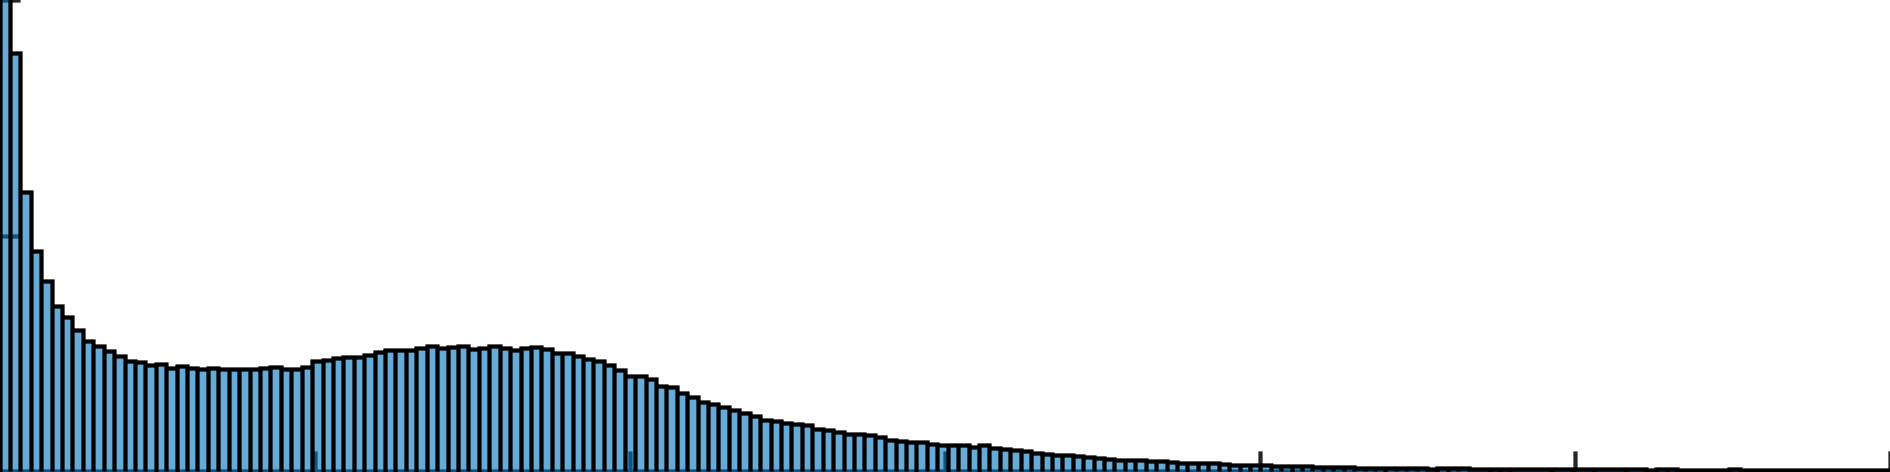
\includegraphics[scale=0.438]{figures/les_zt_040ms_his.png}}  
     \put(44.45,37.4){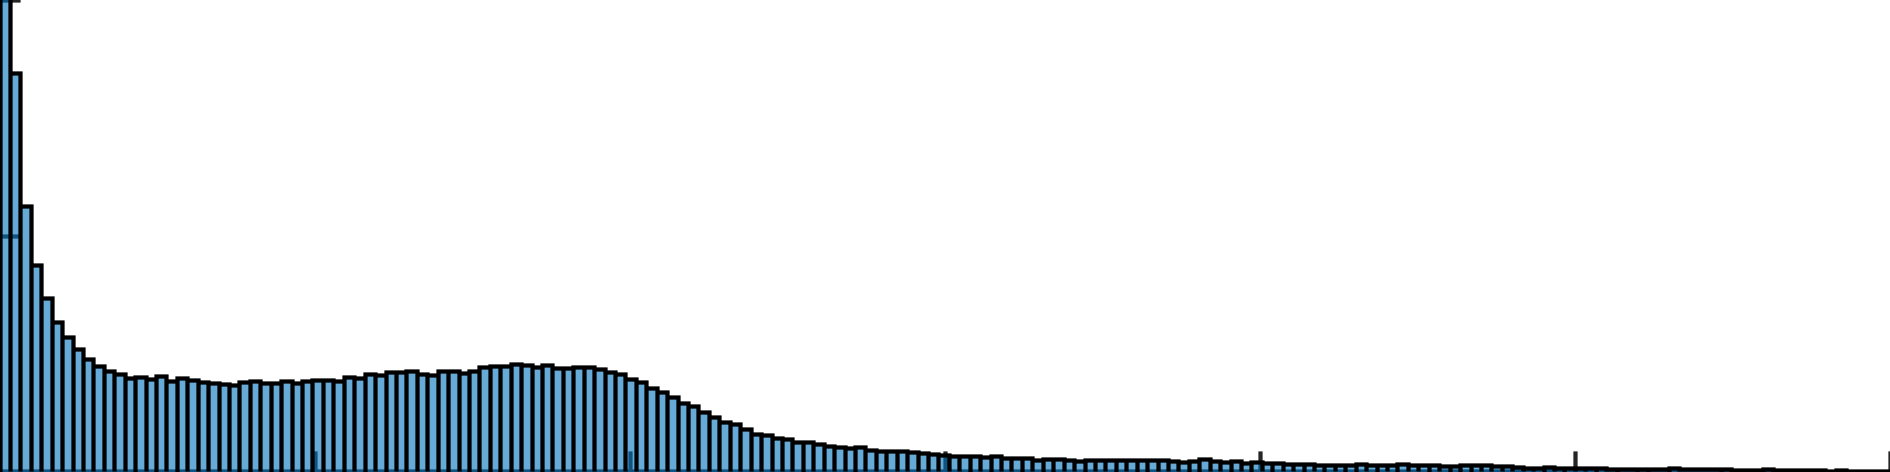
\includegraphics[scale=0.438]{figures/les_zt_044ms_his.png}}  
    
  \end{overpic}
\end{figure}



%%%%%%%%%%%%%%%%%%%%%%%%%%%%%%%%%%%ZT PLANE FIGURE Compare



\begin{figure}[h]	\centering
	\hspace*{-8cm}
	\vspace{5mm}
	\begin{subfigure}{\textwidth}
		\begin{tikzpicture}[>=latex]
		\begin{axis} [
		scale = 0.45,
		scale only axis,        % Plot size does not include axes.
		enlargelimits=false,    % Shrink wrap the PNG.
		height=12cm,
		width=8cm,
		xticklabel style={
			/pgf/number format/fixed,
			/pgf/number format/precision=3
		},
		label style={font=\footnotesize},
		ticklabel style = {font=\scriptsize},
		xtick distance={0.05}, ytick distance={200},
		axis on top,% Axes placed over PNG to avoid obscuring the lines.
		ylabel= Temperature {[K]},
			title=RANS,
		legend style={font=\tiny, draw =none, legend pos=north east,fill=none, legend cell align=left}, 
		]
		\addplot[forget plot] graphics [
		xmin=0, xmax=0.3, 
		ymin=363, ymax=2400] {figures/zt/rans_zt_019ms.png};
		
		\node at (0.075,500) {$Z_{st}$};
		
		\addlegendimage{mark=*, only marks,color={RdGy-4-1}}
		\addlegendentry{Temperature}
		\addlegendimage{color=black,smooth}
		\addlegendentry{$\langle T|Z \rangle$}
		\addlegendimage{color=black,dashed}
		\addlegendentry{Mixing}
		\addlegendimage{color=black,dotted}
		\addlegendentry{Equilibrium}
		

		\node at (0.2,1600) {0.19ms};
		
		\end{axis}
		\hspace{8cm}
	
		\begin{axis} [
		scale = 0.45,
		scale only axis,        % Plot size does not include axes.
		enlargelimits=false,    % Shrink wrap the PNG.
		height=12cm,
		width=8cm,
		xticklabel style={
			/pgf/number format/fixed,
			/pgf/number format/precision=3
		},
		label style={font=\footnotesize},
		ticklabel style = {font=\scriptsize},
		xtick distance={0.05}, ytick distance={200},
		axis on top,% Axes placed over PNG to avoid obscuring the lines.
		ylabel= Temperature {[K]},
			title=LES,
		legend style={font=\tiny, draw =none, legend pos=north east,fill=none, legend cell align=left}, 
		]
		\addplot[forget plot] graphics [
		xmin=0, xmax=0.3, 
		ymin=363, ymax=2400] {figures/zt/les_zt_019ms.png};
		
			
		\node at (0.075,500) {$Z_{st}$};
		
		\addlegendimage{mark=*, only marks,color={RdGy-4-1}}
		\addlegendentry{Temperature}
		\addlegendimage{color=black,smooth}
		\addlegendentry{$\langle T|Z \rangle$}
		\addlegendimage{color=black,dashed}
		\addlegendentry{Mixing}
		\addlegendimage{color=black,dotted}
		\addlegendentry{Equilibrium}
		

		\node at (0.2,1600) {0.19ms};
		
		
		\end{axis}
		\end{tikzpicture}
		
	\end{subfigure}\\
	\hspace*{-8cm}
	\vspace*{5mm}
	\begin{subfigure}{\textwidth}
		\begin{tikzpicture}[>=latex]
		\begin{axis} [
		scale = 0.45,
		scale only axis,        % Plot size does not include axes.
		enlargelimits=false,    % Shrink wrap the PNG.
		height=12cm,
		width=8cm,
		xticklabel style={
			/pgf/number format/fixed,
			/pgf/number format/precision=3
		},
		label style={font=\footnotesize},
		ticklabel style = {font=\scriptsize},
		xtick distance={0.05}, ytick distance={200},
		axis on top,% Axes placed over PNG to avoid obscuring the lines.
		ylabel= Temperature {[K]},
		legend style={font=\tiny, draw =none, legend pos=north east,fill=none, legend cell align=left}, 
		]
		\addplot[forget plot] graphics [
		xmin=0, xmax=0.3, 
		ymin=363, ymax=2400] {figures/zt/rans_zt_039ms.png};
		
		\node at (0.2,2200) {0.39ms};
		
		\end{axis}
		\hspace{8cm}
		\begin{axis} [
	scale = 0.45,
	scale only axis,        % Plot size does not include axes.
	enlargelimits=false,    % Shrink wrap the PNG.
	height=12cm,
	width=8cm,
	xticklabel style={
		/pgf/number format/fixed,
		/pgf/number format/precision=3
	},
	label style={font=\footnotesize},
	ticklabel style = {font=\scriptsize},
	xtick distance={0.05}, ytick distance={200},
	axis on top,% Axes placed over PNG to avoid obscuring the lines.
	ylabel= Temperature {[K]},
	legend style={font=\tiny, draw =none, legend pos=north east,fill=none, legend cell align=left}, 
	]
	\addplot[forget plot] graphics [
	xmin=0, xmax=0.3, 
	ymin=363, ymax=2400] {figures/zt/les_zt_040ms.png};
	
	\node at (0.2,2200) {0.40ms};
	
	\end{axis}
		\end{tikzpicture}
		
	\end{subfigure}\\

	\hspace*{-8cm}
	\vspace{5mm}
	\begin{subfigure}{\textwidth}
		\begin{tikzpicture}[>=latex]
		\begin{axis} [
		scale = 0.45,
		scale only axis,        % Plot size does not include axes.
		enlargelimits=false,    % Shrink wrap the PNG.
		height=12cm,
		width=8cm,
		xticklabel style={
			/pgf/number format/fixed,
			/pgf/number format/precision=3
		},
		label style={font=\footnotesize},
		ticklabel style = {font=\scriptsize},
		xtick distance={0.05}, ytick distance={200},
		axis on top,% Axes placed over PNG to avoid obscuring the lines.
		ylabel= Temperature {[K]},
		xlabel= {$Z$ [-]},
		legend style={font=\tiny, draw =none, legend pos=north east,fill=none, legend cell align=left}, 
		]
		\addplot[forget plot] graphics [
		xmin=0, xmax=0.3, 
		ymin=363, ymax=2400] {figures/zt/rans_zt_045ms.png};
		
		\node at (0.2,2200) {0.44ms};
		
		\end{axis}
		\hspace{8cm}
		\begin{axis} [
	scale = 0.45,
	scale only axis,        % Plot size does not include axes.
	enlargelimits=false,    % Shrink wrap the PNG.
	height=12cm,
	width=8cm,
	xticklabel style={
		/pgf/number format/fixed,
		/pgf/number format/precision=3
	},
	label style={font=\footnotesize},
	ticklabel style = {font=\scriptsize},
	xtick distance={0.05}, ytick distance={200},
	axis on top,% Axes placed over PNG to avoid obscuring the lines.
	ylabel= Temperature {[K]},
	xlabel= {$Z$ [-]},
	legend style={font=\tiny, draw =none, legend pos=north east,fill=none, legend cell align=left}, 
	]
	\addplot[forget plot] graphics [
	xmin=0, xmax=0.3, 
	ymin=363, ymax=2400] {figures/zt/les_zt_044ms.png};
	
	\node at (0.2,2200) {0.44ms};
	
	\end{axis}
		\end{tikzpicture}
		
	\end{subfigure}
	
	
\end{figure}






%%%%%%%%%%%%%%%%%%%%%%%%%%%%%%%%%%%%%%%%%%%%%%%%%%%%%%%%%%%%%%%%%%%%%%%%%%%%%%%%%%%%%%%%%%%%%%%%%%%%%%%%%%%%%%%%%%%%%%%%ZT PLANE FIGURE Compare

%
%
%\begin{figure}[h]	\centering
%	\hspace*{-8cm}
%	\begin{subfigure}{\textwidth}
%		\begin{tikzpicture}[>=latex]
%		\begin{axis} [
%		scale = 0.45,
%		scale only axis,        % Plot size does not include axes.
%		enlargelimits=false,    % Shrink wrap the PNG.
%		height=12cm,
%		width=8cm,
%		xticklabel style={
%			/pgf/number format/fixed,
%			/pgf/number format/precision=3
%		},
%		label style={font=\footnotesize},
%		ticklabel style = {font=\scriptsize},
%		xtick distance={0.05}, ytick distance={200},
%		axis on top,% Axes placed over PNG to avoid obscuring the lines.
%		ylabel= Temperature {[K]},
%		xlabel= {$Z$ [-]},
%			title=RANS,
%		legend style={font=\tiny, draw =none, legend pos=north east,fill=none, legend cell align=left}, 
%		]
%		\addplot[forget plot] graphics [
%		xmin=0, xmax=0.3, 
%		ymin=363, ymax=2400] {figures/Chapter7/spray_data/leszt/rans_zt_019ms.png};
%		
%		\node at (0.075,500) {$Z_{st}$};
%		
%		\addlegendimage{mark=*, only marks,color={RdGy-4-1}}
%		\addlegendentry{Temperature}
%		\addlegendimage{color=black,smooth}
%		\addlegendentry{$\langle T|Z \rangle$}
%		\addlegendimage{color=black,dashed}
%		\addlegendentry{Mixing}
%		\addlegendimage{color=black,dotted}
%		\addlegendentry{Equilibrium}
%		
%
%		\node at (0.2,1600) {0.19ms};
%		
%		\end{axis}
%		\hspace{8cm}
%	
%		\begin{axis} [
%		scale = 0.45,
%		scale only axis,        % Plot size does not include axes.
%		enlargelimits=false,    % Shrink wrap the PNG.
%		height=12cm,
%		width=8cm,
%		xticklabel style={
%			/pgf/number format/fixed,
%			/pgf/number format/precision=3
%		},
%		label style={font=\footnotesize},
%		ticklabel style = {font=\scriptsize},
%		xtick distance={0.05}, ytick distance={200},
%		axis on top,% Axes placed over PNG to avoid obscuring the lines.
%		ylabel= Temperature {[K]},
%		xlabel= {$Z$ [-]},
%			title=LES,
%		legend style={font=\tiny, draw =none, legend pos=north east,fill=none, legend cell align=left}, 
%		]
%		\addplot[forget plot] graphics [
%		xmin=0, xmax=0.3, 
%		ymin=363, ymax=2400] {figures/Chapter7/spray_data/leszt/les_zt_019ms.png};
%		
%			
%		\node at (0.075,500) {$Z_{st}$};
%		
%		\addlegendimage{mark=*, only marks,color={RdGy-4-1}}
%		\addlegendentry{Temperature}
%		\addlegendimage{color=black,smooth}
%		\addlegendentry{$\langle T|Z \rangle$}
%		\addlegendimage{color=black,dashed}
%		\addlegendentry{Mixing}
%		\addlegendimage{color=black,dotted}
%		\addlegendentry{Equilibrium}
%		
%
%		\node at (0.2,1600) {0.19ms};
%		
%		
%		\end{axis}
%		\end{tikzpicture}
%		
%	\end{subfigure}\\
%	\hspace*{-8cm}
%	\begin{subfigure}{\textwidth}
%		\begin{tikzpicture}[>=latex]
%		\begin{axis} [
%		scale = 0.45,
%		scale only axis,        % Plot size does not include axes.
%		enlargelimits=false,    % Shrink wrap the PNG.
%		height=12cm,
%		width=8cm,
%		xticklabel style={
%			/pgf/number format/fixed,
%			/pgf/number format/precision=3
%		},
%		label style={font=\footnotesize},
%		ticklabel style = {font=\scriptsize},
%		xtick distance={0.05}, ytick distance={200},
%		axis on top,% Axes placed over PNG to avoid obscuring the lines.
%		ylabel= Temperature {[K]},
%		xlabel= {$Z$ [-]},
%		legend style={font=\tiny, draw =none, legend pos=north east,fill=none, legend cell align=left}, 
%		]
%		\addplot[forget plot] graphics [
%		xmin=0, xmax=0.3, 
%		ymin=363, ymax=2400] {figures/Chapter7/spray_data/leszt/rans_zt_039ms.png};
%		
%		\node at (0.2,2200) {0.39ms};
%		
%		\end{axis}
%		\hspace{8cm}
%		\begin{axis} [
%	scale = 0.45,
%	scale only axis,        % Plot size does not include axes.
%	enlargelimits=false,    % Shrink wrap the PNG.
%	height=12cm,
%	width=8cm,
%	xticklabel style={
%		/pgf/number format/fixed,
%		/pgf/number format/precision=3
%	},
%	label style={font=\footnotesize},
%	ticklabel style = {font=\scriptsize},
%	xtick distance={0.05}, ytick distance={200},
%	axis on top,% Axes placed over PNG to avoid obscuring the lines.
%	ylabel= Temperature {[K]},
%	xlabel= {$Z$ [-]},
%	legend style={font=\tiny, draw =none, legend pos=north east,fill=none, legend cell align=left}, 
%	]
%	\addplot[forget plot] graphics [
%	xmin=0, xmax=0.3, 
%	ymin=363, ymax=2400] {figures/Chapter7/spray_data/leszt/les_zt_040ms.png};
%	
%	\node at (0.2,2200) {0.40ms};
%	
%	\end{axis}
%		\end{tikzpicture}
%		
%	\end{subfigure}\\
%
%	\hspace*{-8cm}
%	\begin{subfigure}{\textwidth}
%		\begin{tikzpicture}[>=latex]
%		\begin{axis} [
%		scale = 0.45,
%		scale only axis,        % Plot size does not include axes.
%		enlargelimits=false,    % Shrink wrap the PNG.
%		height=12cm,
%		width=8cm,
%		xticklabel style={
%			/pgf/number format/fixed,
%			/pgf/number format/precision=3
%		},
%		label style={font=\footnotesize},
%		ticklabel style = {font=\scriptsize},
%		xtick distance={0.05}, ytick distance={200},
%		axis on top,% Axes placed over PNG to avoid obscuring the lines.
%		ylabel= Temperature {[K]},
%		xlabel= {$Z$ [-]},
%		legend style={font=\tiny, draw =none, legend pos=north east,fill=none, legend cell align=left}, 
%		]
%		\addplot[forget plot] graphics [
%		xmin=0, xmax=0.3, 
%		ymin=363, ymax=2400] {figures/Chapter7/spray_data/leszt/rans_zt_045ms.png};
%		
%		\node at (0.2,2200) {0.44ms};
%		
%		\end{axis}
%		\hspace{8cm}
%		\begin{axis} [
%	scale = 0.45,
%	scale only axis,        % Plot size does not include axes.
%	enlargelimits=false,    % Shrink wrap the PNG.
%	height=12cm,
%	width=8cm,
%	xticklabel style={
%		/pgf/number format/fixed,
%		/pgf/number format/precision=3
%	},
%	label style={font=\footnotesize},
%	ticklabel style = {font=\scriptsize},
%	xtick distance={0.05}, ytick distance={200},
%	axis on top,% Axes placed over PNG to avoid obscuring the lines.
%	ylabel= Temperature {[K]},
%	xlabel= {$Z$ [-]},
%	legend style={font=\tiny, draw =none, legend pos=north east,fill=none, legend cell align=left}, 
%	]
%	\addplot[forget plot] graphics [
%	xmin=0, xmax=0.3, 
%	ymin=363, ymax=2400] {figures/Chapter7/spray_data/leszt/les_zt_044ms.png};
%	
%	\node at (0.2,2200) {0.44ms};
%	
%	\end{axis}
%		\end{tikzpicture}
%		\caption{Temporal evolution of scatter plot of temperature versus mixture fraction between RANS (left) and LES (right) for the 900K \textquotedblleft Spray A\textquotedblright \hspace{1mm}baseline condition.\label{fig:zt_ignition_rans_les}}
%		
%	\end{subfigure}
%	
%	
%\end{figure}

\thispagestyle{empty}
%%%%%%%%%%%%%%%%%%%%%%%%%%%%%%%%%%%%%%%%%%%%%%%%%%%%%%%%%%%%%%%%%%%%%%%%%%%%%%%%%%%%%%%%%%%%%%%%%%%%%%%%%%%%%%%%%%%%%%ZT PLANE FIGURE 
%
%
%
% \begin{figure}[h]	\centering
% 	\hspace*{-10cm}
% 	\begin{subfigure}{\textwidth}
% 		\begin{tikzpicture}[>=latex]
% 		\begin{axis} [
% 		scale = 0.45,
% 		scale only axis,        % Plot size does not include axes.
% 		enlargelimits=false,    % Shrink wrap the PNG.
% 		height=12cm,
% 		width=8cm,
% 		xticklabel style={
% 			/pgf/number format/fixed,
% 			/pgf/number format/precision=3
% 		},
% 		label style={font=\footnotesize},
% 		ticklabel style = {font=\scriptsize},
% 		xtick distance={0.05}, ytick distance={200},
% 		axis on top,% Axes placed over PNG to avoid obscuring the lines.
% 		ylabel= Temperature {[K]},
% 		xlabel= {$Z$ [-]},
% 		legend style={font=\tiny, draw =none, legend pos=north east,fill=none, legend cell align=left}, 
% 		]
% 		\addplot[forget plot] graphics [
% 		xmin=0, xmax=0.3, 
% 		ymin=363, ymax=2400] {figures/Chapter7/spray_data/leszt/les_zt_019ms.png};
		
% 		\node at (0.075,500) {$Z_{st}$};
		
% 		\addlegendimage{mark=*, only marks,color={RdGy-4-1}}
% 		\addlegendentry{Temperature}
% 		\addlegendimage{color=black,smooth}
% 		\addlegendentry{$\langle T|Z \rangle$}
% 		\addlegendimage{color=black,dashed}
% 		\addlegendentry{Mixing}
% 		\addlegendimage{color=black,dotted}
% 		\addlegendentry{Equilibrium}
		
% 		\draw [<-, thick] (0.05,1000) to (0.075,1200);
% 		\node at (0.08,1300) {i};
		
% 		\node at (0.2,1600) {0.19 ms};
		
% 		\end{axis}
% 		\hspace{5.25cm}
% 		\begin{axis} [
% 		scale = 0.425,
% 		scale only axis,        % Plot size does not include axes.
% 		axis on top,
% 		enlargelimits=false,    % Shrink wrap the PNG.
% 		height=12cm,
% 		width=4cm,
% 		title = { $\mathsf{CH_{2}O} \cdot 10^{-3}$ [-]}, 
% 		title style = {font=\scriptsize},
% 		xlabel = {$y$ [mm]},
% 		ylabel = {$x$ [mm]},
% 		xtick distance={5}, ytick distance={10},
% 		label style={font=\footnotesize},
% 		ticklabel style = {font=\scriptsize},
% 		%xticklabels=,,
% 		%yticklabels=,,
% 		colormap name=spectral,
% 		colorbar, % horizontal,
% 		colorbar/width=2.0mm,
% 		point meta min=0,
% 		point meta max=8,
% 		colorbar style={
% 			at={(1.1,1)},
% 			yticklabel style = {font=\scriptsize},
% 		}
% 		]
% 		\addplot graphics [
% 		xmin=-10, xmax=10, 
% 		ymin=0, ymax=60,
% 		] {figures/Chapter7/spray_data/leszt/les_ych2o_019ms.png};
% 		\end{axis}
% 		\hspace{2.6cm}
% 		\begin{axis} [
% 		scale = 0.425,
% 		scale only axis,        % Plot size does not include axes.
% 		enlargelimits=false,    % Shrink wrap the PNG.
% 		height=12cm,
% 		width=4cm,
% 		xlabel = {$y$ [mm]},
% 		xtick distance={5}, 
% 		yticklabels=,,
% 			label style={font=\footnotesize},
% 		ticklabel style = {font=\scriptsize},
% 		title = { $\mathsf{H_{2}O_{2}} \cdot 10^{-3}$ [-]}, 
% 		title style = {font=\scriptsize},
% 		colormap name=spectral,
% 		colorbar,
% 		colorbar/width=2.0mm,
% 		point meta min=0,
% 		point meta max=5,
% 		colorbar style={
% 			at={(1.1,1)},
% 			yticklabel style = {font=\scriptsize},
% 		}
% 		]
% 		\addplot graphics [
% 		xmin=-10, xmax=10, 
% 		ymin=0, ymax=60,
% 		] {figures/Chapter7/spray_data/leszt/les_yh2o2_019ms.png};
% 		\end{axis}
% 		\hspace{2.6cm}
% 		\begin{axis} [
% 		scale = 0.425,
% 		scale only axis,        % Plot size does not include axes.
% 		enlargelimits=false,    % Shrink wrap the PNG.
% 		height=12cm,
% 		width=4cm,
% 				xlabel = {$y$ [mm]},
% 		xtick distance={5}, 
% 		yticklabels=,,
% 			label style={font=\footnotesize},
% 		ticklabel style = {font=\scriptsize},
% 		title = { $\mathsf{OH} \cdot 10^{-5}$ [-]}, 
% 		title style = {font=\scriptsize},
% 		colormap name=spectral,
% 		colorbar,
% 		colorbar/width=2.0mm,
% 		point meta min=0,
% 		point meta max=5,
% 		colorbar style={
% 			at={(1.1,1)},
% 			yticklabel style = {font=\scriptsize},
% 		}
% 		]
% 		\addplot graphics [
% 		xmin=-10, xmax=10, 
% 		ymin=0, ymax=60,
% 		] {figures/Chapter7/spray_data/leszt/les_yoh_019ms.png};
% 		\end{axis}
% 		\end{tikzpicture}

% 		\end{subfigure}\\
% \hspace*{-10cm}
% \begin{subfigure}{\textwidth}
% 	\begin{tikzpicture}[>=latex]
% 	\begin{axis} [
% 	scale = 0.45,
% 	scale only axis,        % Plot size does not include axes.
% 	enlargelimits=false,    % Shrink wrap the PNG.
% 	height=12cm,
% 	width=8cm,
% 	xticklabel style={
% 		/pgf/number format/fixed,
% 		/pgf/number format/precision=3
% 	},
% 	label style={font=\footnotesize},
% 	ticklabel style = {font=\scriptsize},
% 	xtick distance={0.05}, ytick distance={200},
% 	axis on top,% Axes placed over PNG to avoid obscuring the lines.
% 	ylabel= Temperature {[K]},
% 	xlabel= {$Z$ [-]},
% 	legend style={font=\tiny, draw =none, legend pos=north east,fill=none, legend cell align=left}, 
% 	]
% 	\addplot[forget plot] graphics [
% 	xmin=0, xmax=0.3, 
% 	ymin=363, ymax=2400] {figures/Chapter7/spray_data/leszt/les_zt_030ms.png};
	
% 	\node at (0.175,1100) {ii};	
% 	\node at (0.2,2200) {0.30 ms};
	
% 	\end{axis}
% 	\hspace{5.25cm}
% 	\begin{axis} [
% 	scale = 0.425,
% 	scale only axis,        % Plot size does not include axes.
% 	axis on top,
% 	enlargelimits=false,    % Shrink wrap the PNG.
% 	height=12cm,
% 	width=4cm,
% 	title = { $\mathsf{CH_{2}O} \cdot 10^{-3}$ [-]}, 
% 	title style = {font=\scriptsize},
% 	xlabel = {$y$ [mm]},
% 	ylabel = {$x$ [mm]},
% 	xtick distance={5}, ytick distance={10},
% 	label style={font=\footnotesize},
% 	ticklabel style = {font=\scriptsize},
% 	%xticklabels=,,
% 	%yticklabels=,,
% 	colormap name=spectral,
% 	colorbar, % horizontal,
% 	colorbar/width=2.0mm,
% 	point meta min=0,
% 	point meta max=8,
% 	colorbar style={
% 		at={(1.1,1)},
% 		yticklabel style = {font=\scriptsize},
% 	}
% 	]
% 	\addplot graphics [
% 	xmin=-10, xmax=10, 
% 	ymin=0, ymax=60,
% 	] {figures/Chapter7/spray_data/leszt/les_ych2o_030ms.png};
% 	\end{axis}
% 	\hspace{2.6cm}
% 	\begin{axis} [
% 	scale = 0.425,
% 	scale only axis,        % Plot size does not include axes.
% 	enlargelimits=false,    % Shrink wrap the PNG.
% 	height=12cm,
% 	width=4cm,
% 			xlabel = {$y$ [mm]},
% 	xtick distance={5}, 
% 	yticklabels=,,
% 		label style={font=\footnotesize},
% 	ticklabel style = {font=\scriptsize},
% 	title = { $\mathsf{H_{2}O_{2}} \cdot 10^{-3}$ [-]}, 
% 	title style = {font=\scriptsize},
% 	colormap name=spectral,
% 	colorbar,
% 	colorbar/width=2.0mm,
% 	point meta min=0,
% 	point meta max=5,
% 	colorbar style={
% 		at={(1.1,1)},
% 		yticklabel style = {font=\scriptsize},
% 	}
% 	]
% 	\addplot graphics [
% 	xmin=-10, xmax=10, 
% 	ymin=0, ymax=60,
% 	] {figures/Chapter7/spray_data/leszt/les_yh2o2_030ms.png};
% 	\end{axis}
% 	\hspace{2.6cm}
% 	\begin{axis} [
% 	scale = 0.425,
% 	scale only axis,        % Plot size does not include axes.
% 	enlargelimits=false,    % Shrink wrap the PNG.
% 	height=12cm,
% 	width=4cm,
% 		xlabel = {$y$ [mm]},
% xtick distance={5}, 
% 	yticklabels=,,
% 		label style={font=\footnotesize},
% 	ticklabel style = {font=\scriptsize},
% 	title = { $\mathsf{OH} \cdot 10^{-5}$ [-]}, 
% 	title style = {font=\scriptsize},
% 	colormap name=spectral,
% 	colorbar,
% 	colorbar/width=2.0mm,
% 	point meta min=0,
% 	point meta max=5,
% 	colorbar style={
% 		at={(1.1,1)},
% 		yticklabel style = {font=\scriptsize},
% 	}
% 	]
% 	\addplot graphics [
% 	xmin=-10, xmax=10, 
% 	ymin=0, ymax=60,
% 	] {figures/Chapter7/spray_data/leszt/les_yoh_030ms.png};
% 	\end{axis}
% 	\end{tikzpicture}
	
% \end{subfigure}\\
% %\hspace*{-12cm}
% %	\begin{subfigure}{1\textwidth}
% %		\begin{tikzpicture}[>=latex]
% %		\begin{axis} [
% %		scale = 0.45,
% %		scale only axis,        % Plot size does not include axes.
% %		enlargelimits=false,    % Shrink wrap the PNG.
% %		height=12cm,
% %		width=8cm,
% %		xticklabel style={
% %			/pgf/number format/fixed,
% %			/pgf/number format/precision=3
% %		},
% %		label style={font=\footnotesize},
% %		ticklabel style = {font=\scriptsize},
% %		xtick distance={0.05}, ytick distance={200},
% %		axis on top,% Axes placed over PNG to avoid obscuring the lines.
% %		ylabel= Temperature {[K]},
% %		xlabel= {$Z$ [-]},
% %		legend style={font=\tiny, draw =none, legend pos=north east,fill=none, legend cell align=left}, 
% %		]
% %		\addplot[forget plot] graphics [
% %		xmin=0, xmax=0.3, 
% %		ymin=363, ymax=2400] {figures/Chapter7/spray_data/leszt/les_zt_040ms.png};
% %		
% %		\draw [<-, thick] (0.175,1100) to (0.175,1200);
% %	\draw [<-, thick] (0.125,1300) to (0.155,1300);
% %	\node at (0.175,1300) {iii};
% %		\node at (0.2,2200) {0.40ms};
% %		
% %		\end{axis}
% %		\hspace{5.25cm}
% %		\begin{axis} [
% %		scale = 0.425,
% %		scale only axis,        % Plot size does not include axes.
% %		axis on top,
% %		enlargelimits=false,    % Shrink wrap the PNG.
% %		height=12cm,
% %		width=4cm,
% %		title = { $\mathsf{CH_{2}O} \cdot 10^{-3}$ [-]}, 
% %		title style = {font=\scriptsize},
% %		xlabel = {$y$ [mm]},
% %		ylabel = {$x$ [mm]},
% %		xtick distance={5}, ytick distance={10},
% %		label style={font=\footnotesize},
% %		ticklabel style = {font=\scriptsize},
% %		%xticklabels=,,
% %		%yticklabels=,,
% %		colormap name=spectral,
% %		colorbar, % horizontal,
% %		colorbar/width=2.0mm,
% %		point meta min=0,
% %		point meta max=8,
% %		colorbar style={
% %			at={(1.1,1)},
% %			yticklabel style = {font=\scriptsize},
% %		}
% %		]
% %		\addplot graphics [
% %		xmin=-10, xmax=10, 
% %		ymin=0, ymax=60,
% %		] {figures/Chapter7/spray_data/leszt/les_ych2o_040ms.png};
% %		\end{axis}
% %		\hspace{2.6cm}
% %		\begin{axis} [
% %		scale = 0.425,
% %		scale only axis,        % Plot size does not include axes.
% %		enlargelimits=false,    % Shrink wrap the PNG.
% %		height=12cm,
% %		width=4cm,
% %		xticklabels=,,
% %		yticklabels=,,
% %		title = { $\mathsf{H_{2}O_{2}} \cdot 10^{-3}$ [-]}, 
% %		title style = {font=\scriptsize},
% %		colormap name=spectral,
% %		colorbar,
% %		colorbar/width=2.0mm,
% %		point meta min=0,
% %		point meta max=5,
% %		colorbar style={
% %			at={(1.1,1)},
% %			yticklabel style = {font=\scriptsize},
% %		}
% %		]
% %		\addplot graphics [
% %		xmin=-10, xmax=10, 
% %		ymin=0, ymax=60,
% %		] {figures/Chapter7/spray_data/leszt/les_yh2o2_040ms.png};
% %		\end{axis}
% %		\hspace{2.6cm}
% %		\begin{axis} [
% %		scale = 0.425,
% %		scale only axis,        % Plot size does not include axes.
% %		enlargelimits=false,    % Shrink wrap the PNG.
% %		height=12cm,
% %		width=4cm,
% %		xticklabels=,,
% %		yticklabels=,,
% %		title = { $\mathsf{OH} \cdot 10^{-5}$ [-]}, 
% %		title style = {font=\scriptsize},
% %		colormap name=spectral,
% %		colorbar,
% %		colorbar/width=2.0mm,
% %		point meta min=0,
% %		point meta max=5,
% %		colorbar style={
% %			at={(1.1,1)},
% %			yticklabel style = {font=\scriptsize},
% %		}
% %		]
% %		\addplot graphics [
% %		xmin=-10, xmax=10, 
% %		ymin=0, ymax=60,
% %		] {figures/Chapter7/spray_data/leszt/les_yoh_040ms.png};
% %		\end{axis}
% %		\end{tikzpicture}
% %
% %	\end{subfigure}\\
% %
% \hspace*{-10cm}
% \begin{subfigure}{\textwidth}
% 	\begin{tikzpicture}[>=latex]
% 	\begin{axis} [
% 	scale = 0.45,
% 	scale only axis,        % Plot size does not include axes.
% 	enlargelimits=false,    % Shrink wrap the PNG.
% 	height=12cm,
% 	width=8cm,
% 	xticklabel style={
% 		/pgf/number format/fixed,
% 		/pgf/number format/precision=3
% 	},
% 	label style={font=\footnotesize},
% 	ticklabel style = {font=\scriptsize},
% 	xtick distance={0.05}, ytick distance={200},
% 	axis on top,% Axes placed over PNG to avoid obscuring the lines.
% 	ylabel= Temperature {[K]},
% 	xlabel= {$Z$ [-]},
% 	legend style={font=\tiny, draw =none, legend pos=north east,fill=none, legend cell align=left}, 
% 	]
% 	\addplot[forget plot] graphics [
% 	xmin=0, xmax=0.3, 
% 	ymin=363, ymax=2400] {figures/Chapter7/spray_data/leszt/les_zt_044ms.png};
% 	\node at (0.2,2200) {0.44 ms};
% \draw [->, thick] (0.12,1200) to (0.08,1500);
% \node at (0.12,1150) {iii};
	
% 	\end{axis}
% 	\hspace{5.25cm}
% 	\begin{axis} [
% 	scale = 0.425,
% 	scale only axis,        % Plot size does not include axes.
% 	axis on top,
% 	enlargelimits=false,    % Shrink wrap the PNG.
% 	height=12cm,
% 	width=4cm,
% 	title = { $\mathsf{CH_{2}O} \cdot 10^{-3}$ [-]}, 
% 	title style = {font=\scriptsize},
% 	xlabel = {$y$ [mm]},
% 	ylabel = {$x$ [mm]},
% 	xtick distance={5}, ytick distance={10},
% 	label style={font=\footnotesize},
% 	ticklabel style = {font=\scriptsize},
% 	%xticklabels=,,
% 	%yticklabels=,,
% 	colormap name=spectral,
% 	colorbar, % horizontal,
% 	colorbar/width=2.0mm,
% 	point meta min=0,
% 	point meta max=8,
% 	colorbar style={
% 		at={(1.1,1)},
% 		yticklabel style = {font=\scriptsize},
% 	}
% 	]
% 	\addplot graphics [
% 	xmin=-10, xmax=10, 
% 	ymin=0, ymax=60,
% 	] {figures/Chapter7/spray_data/leszt/les_ych2o_044ms.png};
% 	\end{axis}
% 	\hspace{2.6cm}
% 	\begin{axis} [
% 	scale = 0.425,
% 	scale only axis,        % Plot size does not include axes.
% 	enlargelimits=false,    % Shrink wrap the PNG.
% 	height=12cm,
% 	width=4cm,
% 			xlabel = {$y$ [mm]},
% 	xtick distance={5}, 
% 	yticklabels=,,
% 		label style={font=\footnotesize},
% 	ticklabel style = {font=\scriptsize},
% 	title = { $\mathsf{H_{2}O_{2}} \cdot 10^{-3}$ [-]}, 
% 	title style = {font=\scriptsize},
% 	colormap name=spectral,
% 	colorbar,
% 	colorbar/width=2.0mm,
% 	point meta min=0,
% 	point meta max=5,
% 	colorbar style={
% 		at={(1.1,1)},
% 		yticklabel style = {font=\scriptsize},
% 	}
% 	]
% 	\addplot graphics [
% 	xmin=-10, xmax=10, 
% 	ymin=0, ymax=60,
% 	] {figures/Chapter7/spray_data/leszt/les_yh2o2_044ms.png};
% 	\end{axis}
% 	\hspace{2.6cm}
% 	\begin{axis} [
% 	scale = 0.425,
% 	scale only axis,        % Plot size does not include axes.
% 	enlargelimits=false,    % Shrink wrap the PNG.
% 	height=12cm,
% 	width=4cm,
% 		xlabel = {$y$ [mm]},
% xtick distance={5}, 
% 	yticklabels=,,
% 		label style={font=\footnotesize},
% 	ticklabel style = {font=\scriptsize},
% 	title = { $\mathsf{OH} \cdot 10^{-5}$ [-]}, 
% 	title style = {font=\scriptsize},
% 	colormap name=spectral,
% 	colorbar,
% 	colorbar/width=2.0mm,
% 	point meta min=0,
% 	point meta max=5,
% 	colorbar style={
% 		at={(1.1,1)},
% 		yticklabel style = {font=\scriptsize},
% 	}
% 	]
% 	\addplot graphics [
% 	xmin=-10, xmax=10, 
% 	ymin=0, ymax=60,
% 	] {figures/Chapter7/spray_data/leszt/les_yoh_044ms.png};
% 	\end{axis}
% 	\end{tikzpicture}
	
% \end{subfigure}
%                                                                                                 
	
% \end{figure}


               %%%%%%%%%%%%%%% begin figure %%%%%%%%%%%%%%%%
\begin{figure}[htb]
	\begin{center}
		\subfigure[]{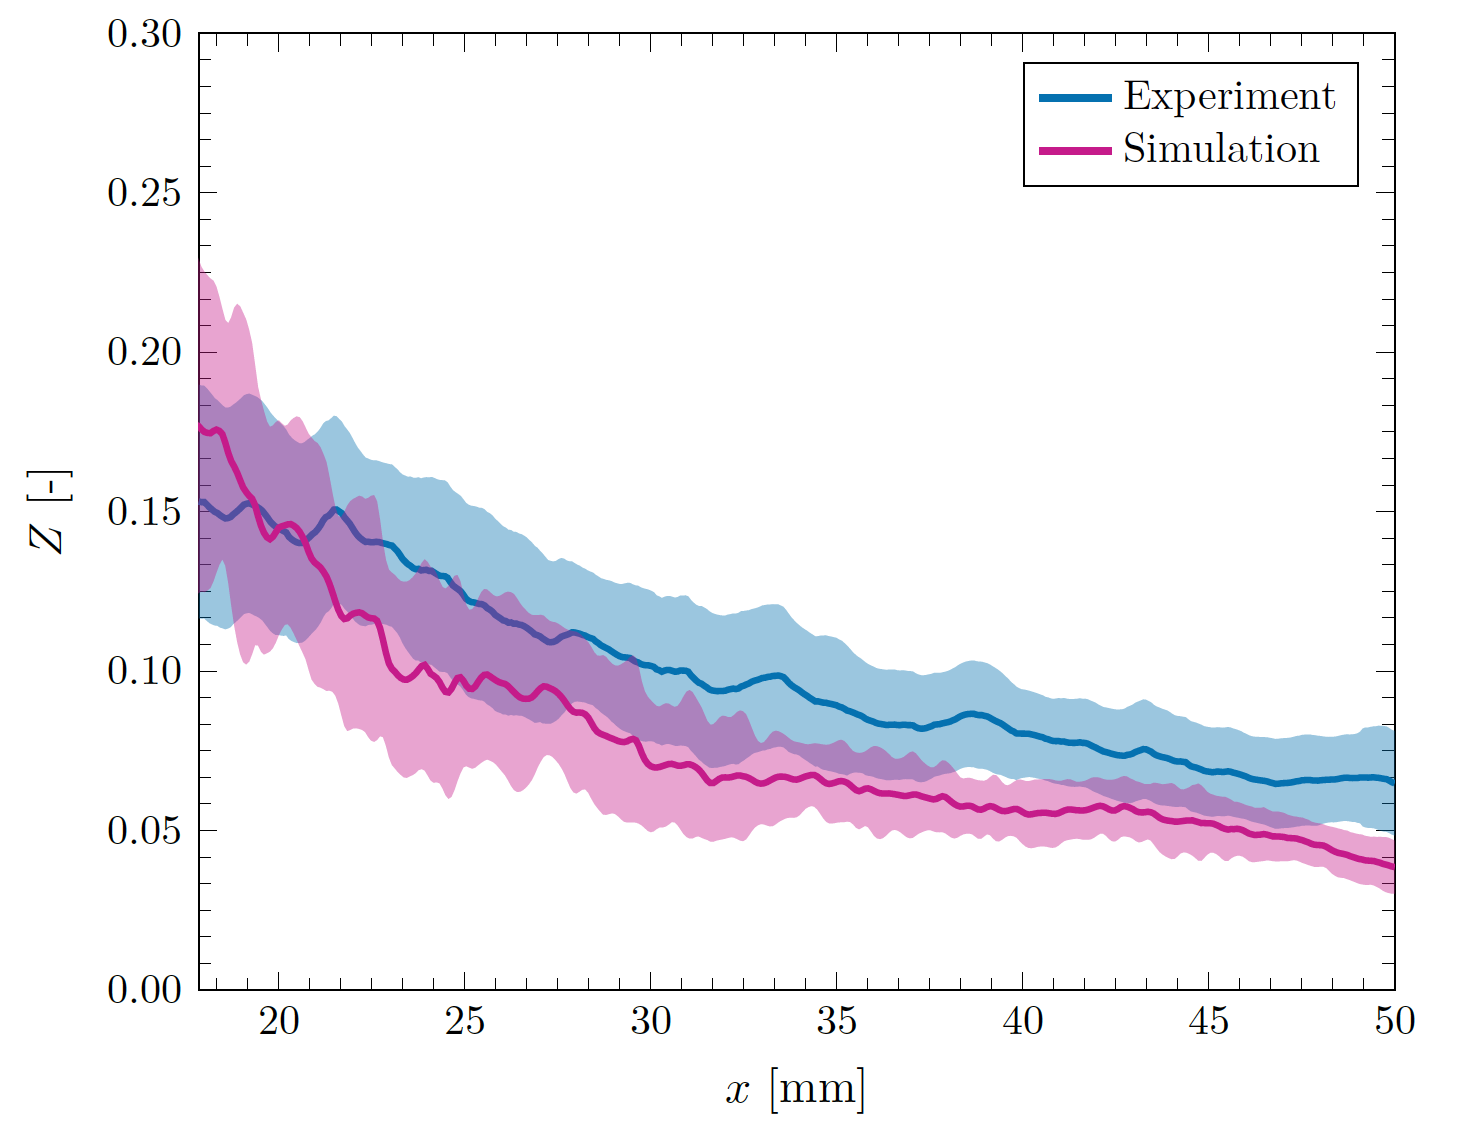
\includegraphics[width=0.5\columnwidth]{figures/axial_mix1.png}}%
		\subfigure[]{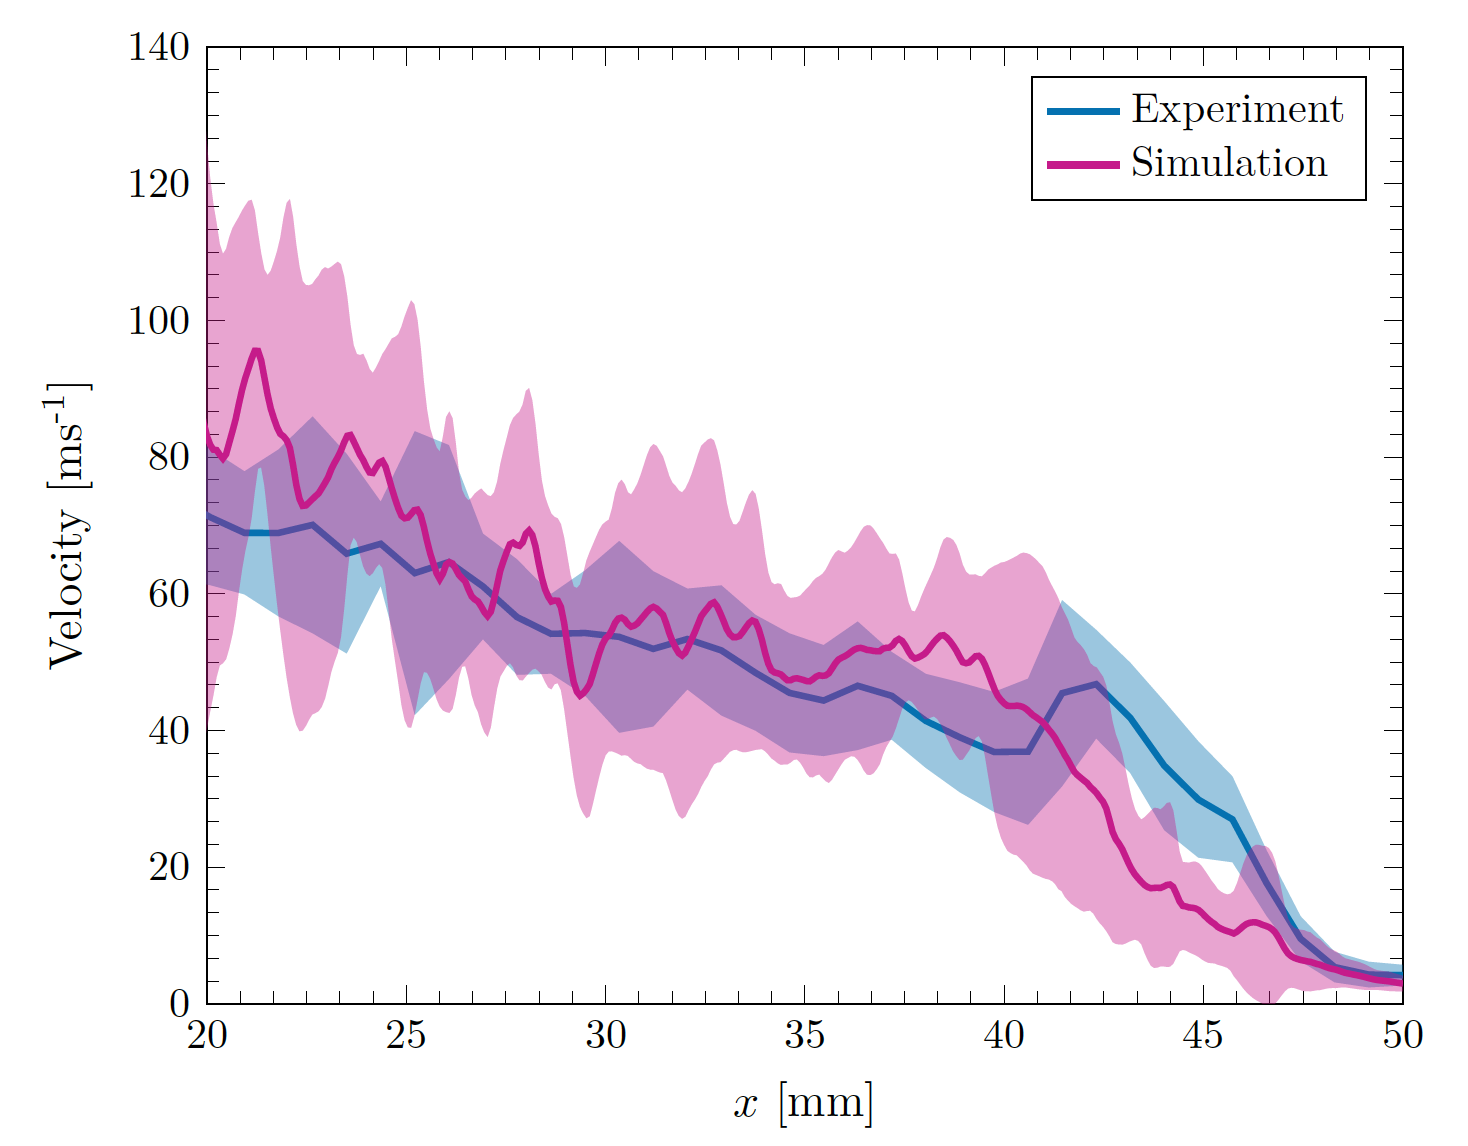
\includegraphics[width=0.5\columnwidth]{figures/axial_vel1.png}}%
		\caption{ Axial comparison of experimental and simulation  (a) mixture fraction distribution and (b) velocity fields at 1.0 ms ASI.  The shaded area represents standard deviation.}
		\label{fig:axial}
	\end{center}
\end{figure}
%%%%%%%%%%%%%%%% end figure %%%%%%%%%%%%%%%%%%                                                                      

% begin{figure}[h]
% 	\centering
% 	\begin{tikzpicture}[>=latex]
% 	\begin{groupplot}[
% 	group style = {group size = 2 by 5, horizontal sep=25pt, vertical sep=5pt},
% 	height = 4cm,
% 	width = 4cm,
% 	scale = 0.85,
% 	scale only axis,        % Plot size does not include axes.
% 	enlargelimits=false,   
% 	%tick label style={/pgf/number format/fixed},
% 	axis on top,
% 	xtick distance={5}, ytick distance={5}
% 	]
% 	%%%
% 	\nextgroupplot[yticklabels={,,},xticklabels={,,},
% 	colorbar horizontal,
% 	colormap name = spectral,
% 	point meta min=550,point meta max=2200,
% 	colorbar/width=2.0mm,
% 	colorbar style={at={(0,1.20)},anchor=north west,
% 	width=1*\pgfkeysvalueof{/pgfplots/parent axis width},
% 	xtick={550,965,1375,1780,2200},
% 	xticklabel style = {font=\tiny},
% 	title={Temperature [K]}}
% 	]
% 	\addplot[forget plot] graphics [
% 	xmin=-10, xmax=10,
% 	ymin=15, ymax=35,
% 	] {figures/spray_data/flol/les_temp_095ms.png};

% 	\draw [color=black,dashed, thick] (-10,18.08) to (10,18.08);
% 	\draw [<-, thick] (-4.0,20) to (-7.0,20);
% 	\node at (-8.0,20) {i};
	
% 	\draw [<-, thick] (-0.75,19) to (5.0,19);
% 	\node at (6.0,19) {A};
	
% 	\nextgroupplot[yticklabels={,,},xticklabels={,,},
% 	colorbar horizontal,
% 	colormap name = spectral,
% 	point meta min=0.01,point meta max=100,
% 	colorbar/width=2.0mm,
% 	colorbar style={at={(0,1.20)},anchor=north west,
% 		width=1*\pgfkeysvalueof{/pgfplots/parent axis width},
% 		xtick={0.01,0.1,1.0,10,100},
% 		xmode=log,
% 		xticklabel style = {font=\scriptsize},
% 		title={$\chi$ [1/s]}}
% 	]
% 	\addplot[forget plot] graphics [
% 	xmin=-10, xmax=10,
% 	ymin=15, ymax=35,
% 	] {figures/spray_data/flol/les_scad_095ms.png};
% 	\draw [color=black,dashed, thick] (-10,18.08) to (10,18.08);
% 	%%%
% 	\nextgroupplot[yticklabels={,,},xticklabels={,,},
% 	]
% 	\addplot[forget plot] graphics [
% 	xmin=-10, xmax=10,
% 	ymin=15, ymax=35,
% 	] {figures/spray_data/flol/les_temp_097ms.png};
% 	\draw [color=black,dashed, thick] (-10,18.08) to (10,18.08);
% 	\draw [<-, thick] (-4.0,20.5) to (-7.0,20.5);
% 	\node at (-8.0,20.5) {ii};
	
% 	\draw [<-, thick] (-0.75,19) to (5.0,19);
% 	\node at (6.0,19) {B};
	
% 	\nextgroupplot[yticklabels={,,},xticklabels={,,},
% 	]
% 	\addplot[forget plot] graphics [
% 	xmin=-10, xmax=10,
% 	ymin=15, ymax=35,
% 	] {figures/spray_data/flol/les_scad_097ms.png};
% 	\draw [color=black,dashed, thick] (-10,18.08) to (10,18.08);
% 	%%%	
% 	\nextgroupplot[yticklabels={,,},xticklabels={,,},
% 	]
% 	\addplot[forget plot] graphics [
% 	xmin=-10, xmax=10,
% 	ymin=15, ymax=35,
% 	] {figures/spray_data/flol/les_temp_099ms.png};
% 	\draw [color=black,dashed, thick] (-10,18.08) to (10,18.08);
% 	\draw [<-, thick] (-3.75,21.75) to (-7.0,23);
% 	\node at (-8.0,23) {iii};
	
% 	\nextgroupplot[yticklabels={,,},xticklabels={,,},
% 	]
% 	\addplot[forget plot] graphics [
% 	xmin=-10, xmax=10,
% 	ymin=15, ymax=35,
% 	] {figures/spray_data/flol/les_scad_099ms.png};
% 	\draw [color=black,dashed, thick] (-10,18.08) to (10,18.08);
% 	%%%	
% 	\nextgroupplot[yticklabels={,,},xticklabels={,,},
% 	]
% 	\addplot[forget plot] graphics [
% 	xmin=-10, xmax=10,
% 	ymin=15, ymax=35,
% 	] {figures/spray_data/flol/les_temp_100ms.png};
% 	\draw [color=black,dashed, thick] (-10,18.08) to (10,18.08);
	
% 	\nextgroupplot[yticklabels={,,},xticklabels={,,},
% 	]
% 	\addplot[forget plot] graphics [
% 	xmin=-10, xmax=10,
% 	ymin=15, ymax=35,
% 	] {figures/spray_data/flol/les_scad_100ms.png};
% 	\draw [color=black,dashed, thick] (-10,18.08) to (10,18.08);
% 	%%%
% 	\nextgroupplot[
% 	xlabel = {$y$ [mm]},
% 	ylabel = {$x$ [mm]},
% 	xtick distance={5}, ytick distance={5}
% 	]
% 	\addplot[forget plot] graphics [
% 	xmin=-10, xmax=10,
% 	ymin=15, ymax=35,
% 	] {figures/spray_data/flol/les_temp_102ms.png};
% 	\draw [color=black,dashed, thick] (-10,18.08) to (10,18.08);
% 	\draw [<-, thick] (-3.75,21.75) to (-7.0,23);
% 	\node at (-8.0,23) {iv};
	
% 	\nextgroupplot[
% 	xlabel = {$y$ [mm]},
% 	%ylabel = {$x$ [mm]},
% 	xtick distance={5}, ytick distance={5}
% 	]
% 	\addplot[forget plot] graphics [
% 	xmin=-10, xmax=10,
% 	ymin=15, ymax=35,
% 	] {figures/spray_data/flol/les_scad_102ms.png};
% 	\draw [color=black,dashed, thick] (-10,18.08) to (10,18.08);
	
% 	\end{groupplot}
	
% 	\node (title) at ($(group c1r1.center)+(-3.75,1.75cm)$) {$t=0.95$ ms};
% 	\node (title) at ($(group c1r2.center)+(-3.75,1.75cm)$) {$t=0.97$ ms};
% 	\node (title) at ($(group c1r3.center)+(-3.75,1.75cm)$) {$t=0.99$ ms};
% 	\node (title) at ($(group c1r4.center)+(-3.75,1.75cm)$) {$t=1.01$ ms};
% 	\node (title) at ($(group c1r5.center)+(-3.75,1.75cm)$) {$t=1.02$ ms};

% 	\end{tikzpicture}
% 	\caption{Temperature (left) and scalar dissipation (right) evolution near the flame lift-off length. The black dashed line marks the simulations flame lift-off length. The solid black line is the contour of stoichiometric mixture fraction.\label{fig:tempscad_les}}
% \end{figure}


% figure
% hold on
% [cs,hc]=contourf(Xq,Rq,phiq,[550:20:2400]); %,[0:1e-4:5e-3]
% colormap('jet')
% %colorbar;
% caxis([550 2400])
% %txt = '0.70 ms';
% %text(1,8,txt,'FontSize',14)
% set(hc,'EdgeColor','none')
% shading interp;
% set(gca, 'Position',[0 0 1 1])
% % colorbar
% % caxis([600 2400])
% axis equal
% axis([0 60 -10 10])
% set(gca,'XTick',0:10:60); 
% set(gca,'YTick',-10:5:10); 
% axis off
% set(gcf, 'Units','centimeters', 'Position',[0 0 12 4]) 

% filename2 = sprintf('LESYao_temp_08ms_plane%d', i) ;
% print( filename2, '-dpng','-r600') ;


\newpage
\pagenumbering{arabic} 


\bibliographystyle{abbrv}
\bibliography{sae_cr}

\end{document}

%%% Local Variables: 
%%% mode: latex
%%% TeX-master: t
%%% End: 